%%% The main file. It contains definitions of basic parameters and includes all other parts.

%% Settings for single-side (simplex) printing
% Margins: left 40mm, right 25mm, top and bottom 25mm
% (but beware, LaTeX adds 1in implicitly)
\documentclass[12pt,a4paper]{report}
\setlength\textwidth{145mm}
\setlength\textheight{247mm}
\setlength\oddsidemargin{15mm}
\setlength\evensidemargin{15mm}
\setlength\topmargin{0mm}
\setlength\headsep{0mm}
\setlength\headheight{0mm}
% \openright makes the following text appear on a right-hand page
\let\openright=\clearpage

%% Settings for two-sided (duplex) printing
% \documentclass[12pt,a4paper,twoside,openright]{report}
% \setlength\textwidth{145mm}
% \setlength\textheight{247mm}
% \setlength\oddsidemargin{14.2mm}
% \setlength\evensidemargin{0mm}
% \setlength\topmargin{0mm}
% \setlength\headsep{0mm}
% \setlength\headheight{0mm}
% \let\openright=\cleardoublepage

%% Generate PDF/A-2u
\usepackage[a-2u]{pdfx}

%% Character encoding: usually latin2, cp1250 or utf8:
\usepackage[utf8]{inputenc}

%% Prefer Latin Modern fonts
\usepackage{lmodern}

%% Further useful packages (included in most LaTeX distributions)
\usepackage{amsmath}        % extensions for typesetting of math
\usepackage{amsfonts}       % math fonts
\usepackage{amsthm}         % theorems, definitions, etc.
\usepackage{bbding}         % various symbols (squares, asterisks, scissors, ...)
\usepackage{bm}             % boldface symbols (\bm)
\usepackage{graphicx}       % embedding of pictures
\usepackage{fancyvrb}       % improved verbatim environment
\usepackage{natbib}         % citation style AUTHOR (YEAR), or AUTHOR [NUMBER]
\usepackage[nottoc]{tocbibind} % makes sure that bibliography and the lists
			    % of figures/tables are included in the table
			    % of contents
\usepackage{dcolumn}        % improved alignment of table columns
\usepackage{booktabs}       % improved horizontal lines in tables
\usepackage{paralist}       % improved enumerate and itemize
\usepackage{xcolor}         % typesetting in color
\usepackage{minted}
\usepackage{forest}
%\usepackage{tabularx}
\usepackage{multirow}
\usepackage{tabularx}

% My includes
\usepackage{listings,xcolor}
\usepackage{inconsolata}

\definecolor{dkgreen}{rgb}{0,.6,0}
\definecolor{dkblue}{rgb}{0,0,.6}
\definecolor{dkyellow}{cmyk}{0,0,.8,.3}

\lstset{
  language        = php,
  basicstyle      = \small\ttfamily,
  keywordstyle    = \color{dkblue},
  stringstyle     = \color{red},
  identifierstyle = \color{dkgreen},
  commentstyle    = \color{gray},
  emph            =[1]{php},
  emphstyle       =[1]\color{black},
  emph            =[2]{if,and,or,else},
  emphstyle       =[2]\color{dkyellow},
  basicstyle=\footnotesize,  
  breaklines=true,
  tabsize=2,
  literate={\ \ }{{\ }}1
}
%%% Basic information on the thesis

% Thesis title in English (exactly as in the formal assignment)
\def\ThesisTitle{Web application for swimming competitions management} %nazev abych vystihnul casovou usporu

% Author of the thesis
\def\ThesisAuthor{Štěpán Klos}

% Year when the thesis is submitted
\def\YearSubmitted{2023}

% Name of the department or institute, where the work was officially assigned
% (according to the Organizational Structure of MFF UK in English,
% or a full name of a department outside MFF)
\def\Department{Department of Software Engineering}

% Is it a department (katedra), or an institute (ústav)?
\def\DeptType{Department}

% Thesis supervisor: name, surname and titles
\def\Supervisor{doc. Mgr. Martin Nečaský, Ph.D.}

% Supervisor's department (again according to Organizational structure of MFF)
\def\SupervisorsDepartment{Software and Data Engineering}

% Study programme and specialization
\def\StudyProgramme{Computer Science}
\def\StudyBranch{Software and Data Engineering}

% An optional dedication: you can thank whomever you wish (your supervisor,
% consultant, a person who lent the software, etc.)
\def\Dedication{%
I would like to thank my supervisor doc. Mgr. Martin Nečaský, Ph.D. for his valuable advice and suggestions. Thanks to his guidance and expertise, I was able to take my knowledge to the next level. Each consultation was very interesting and provided valuable insights from a highly experience person in software engineering that I have internalized and continue to apply in my work.
}

% Abstract (recommended length around 80-200 words; this is not a copy of your thesis assignment!)
\def\Abstract{%
The goal of this project is to streamline the management process for swimming competitions in the Czech Republic. To achieve this, we are developing a system with a user-friendly web interface that is also mobile-friendly. The system will include all necessary infrastructure and utilize a MySQL database for data storage. Backend tasks will be handled by extensible PHP managers. For the frontend, we are implementing a custom drag-and-drop DOM API in JavaScript to improve the user experience.
}

% 3 to 5 keywords (recommended), each enclosed in curly braces
\def\Keywords{%
{key} {web application, web, automation, catalogization, administration, cms, full stack, frontend, backend}
}

%% The hyperref package for clickable links in PDF and also for storing
%% metadata to PDF (including the table of contents).
%% Most settings are pre-set by the pdfx package.
\hypersetup{unicode}
\hypersetup{breaklinks=true}

% Definitions of macros (see description inside)
%%% This file contains definitions of various useful macros and environments %%%
%%% Please add more macros here instead of cluttering other files with them. %%%

%%% Minor tweaks of style

% These macros employ a little dirty trick to convince LaTeX to typeset
% chapter headings sanely, without lots of empty space above them.
% Feel free to ignore.
\makeatletter
\def\@makechapterhead#1{
  {\parindent \z@ \raggedright \normalfont
   \Huge\bfseries \thechapter. #1
   \par\nobreak
   \vskip 20\p@
}}
\def\@makeschapterhead#1{
  {\parindent \z@ \raggedright \normalfont
   \Huge\bfseries #1
   \par\nobreak
   \vskip 20\p@
}}
\makeatother

% This macro defines a chapter, which is not numbered, but is included
% in the table of contents.
\def\chapwithtoc#1{
\chapter*{#1}
\addcontentsline{toc}{chapter}{#1}
}

% Draw black "slugs" whenever a line overflows, so that we can spot it easily.
\overfullrule=1mm

%%% Macros for definitions, theorems, claims, examples, ... (requires amsthm package)

\theoremstyle{plain}
\newtheorem{thm}{Theorem}
\newtheorem{lemma}[thm]{Lemma}
\newtheorem{claim}[thm]{Claim}

\theoremstyle{plain}
\newtheorem{defn}{Definition}

\theoremstyle{remark}
\newtheorem*{cor}{Corollary}
\newtheorem*{rem}{Remark}
\newtheorem*{example}{Example}

%%% An environment for proofs

\newenvironment{myproof}{
  \par\medskip\noindent
  \textit{Proof}.
}{
\newline
\rightline{$\qedsymbol$}
}

%%% An environment for typesetting of program code and input/output
%%% of programs. (Requires the fancyvrb package -- fancy verbatim.)

%%%\DefineVerbatimEnvironment{code}{Verbatim}{fontsize=\small, frame=single}
\renewcommand{\theFancyVerbLine}{\ttfamily \normalfont \arabic{FancyVerbLine}:} %% bigger line numbers

\DefineVerbatimEnvironment{code}{Verbatim}{fontsize=\footnotesize,frame=single, tabsize=4}
\newminted{csharp}{frame=single, linenos, tabsize=4, mathescape=true, fontsize=\footnotesize}
\newminted{php}{
fontfamily=tt,
linenos=true,
breaklines=true,
numberblanklines=true,
numbersep=5pt,
gobble=0,
frame=leftline,
framerule=0.4pt,
framesep=2mm,
funcnamehighlighting=true,
tabsize=4,
obeytabs=false,
mathescape=false
samepage=false, %with this setting you can force the list to appear on the same page
showspaces=false,
showtabs =false,
texcl=false,
}
%%% The field of all real and natural numbers
\newcommand{\R}{\mathbb{R}}
\newcommand{\N}{\mathbb{N}}

%%% Useful operators for statistics and probability
\DeclareMathOperator{\pr}{\textsf{P}}
\DeclareMathOperator{\E}{\textsf{E}\,}
\DeclareMathOperator{\var}{\textrm{var}}
\DeclareMathOperator{\sd}{\textrm{sd}}

%%% Transposition of a vector/matrix
\newcommand{\T}[1]{#1^\top}

%%% Various math goodies
\newcommand{\goto}{\rightarrow}
\newcommand{\gotop}{\stackrel{P}{\longrightarrow}}
\newcommand{\maon}[1]{o(n^{#1})}
\newcommand{\abs}[1]{\left|{#1}\right|}
\newcommand{\dint}{\int_0^\tau\!\!\int_0^\tau}
\newcommand{\isqr}[1]{\frac{1}{\sqrt{#1}}}

%%% Various table goodies
\newcommand{\pulrad}[1]{\raisebox{1.5ex}[0pt]{#1}}
\newcommand{\mc}[1]{\multicolumn{1}{c}{#1}}


% Title page and various mandatory informational pages
\begin{document}
%%% Title page of the thesis and other mandatory pages

%%% Title page of the thesis

\pagestyle{empty}
\hypersetup{pageanchor=false}
\begin{center}

\centerline{\mbox{
\includegraphics[width=166mm]{../img/logo-en.pdf}}}

\vspace{-8mm}
\vfill

{\bf\Large BACHELOR THESIS}

\vfill

{\LARGE\ThesisAuthor}

\vspace{15mm}

{\LARGE\bfseries\ThesisTitle}

\vfill

\Department

\vfill

{
\centerline{\vbox{\halign{\hbox to 0.45\hsize{\hfil #}&\hskip 0.5em\parbox[t]{0.45\hsize}{\raggedright #}\cr
Supervisor of the bachelor thesis:&\Supervisor \cr
\noalign{\vspace{2mm}}
Study programme:&\StudyProgramme \cr
\noalign{\vspace{2mm}}
Study branch:&\StudyBranch \cr
}}}}

\vfill

% Zde doplňte rok
Prague \YearSubmitted

\end{center}

\newpage

%%% Here should be a bound sheet included -- a signed copy of the "bachelor
%%% thesis assignment". This assignment is NOT a part of the electronic
%%% version of the thesis. DO NOT SCAN.

%%%This is not a~part of the electronic version of the thesis, do not scan!}
Sth

%%% A page with a solemn declaration to the bachelor thesis

\openright
\hypersetup{pageanchor=true}
\pagestyle{plain}
\pagenumbering{roman}
\vglue 0pt plus 1fill

\noindent
I declare that I carried out this bachelor thesis independently, and only with the cited
sources, literature and other professional sources. It has not been used to obtain another
or the same degree.

\medskip\noindent
I understand that my work relates to the rights and obligations under the Act No.~121/2000 Sb.,
the Copyright Act, as amended, in particular the fact that the Charles
University has the right to conclude a license agreement on the use of this
work as a school work pursuant to Section 60 subsection 1 of the Copyright~Act.

\vspace{10mm}

\hbox{\hbox to 0.5\hsize{%
In \hbox to 6em{\dotfill} date \hbox to 6em{\dotfill}
\hss}\hbox to 0.5\hsize{\dotfill\quad}}
\smallskip
\hbox{\hbox to 0.5\hsize{}\hbox to 0.5\hsize{\hfil Author's signature\hfil}}

\vspace{20mm}
\newpage

%%% Dedication

\openright

\noindent
\Dedication

\newpage

%%% Mandatory information page of the thesis

\openright

\vbox to 0.5\vsize{
\setlength\parindent{0mm}
\setlength\parskip{5mm}

Title:
\ThesisTitle

Author:
\ThesisAuthor

\DeptType:
\Department

Supervisor:
\Supervisor, \SupervisorsDepartment

Abstract:
\Abstract

Keywords:
\Keywords

\vss}

\newpage

\openright
\pagestyle{plain}
\pagenumbering{arabic}
\setcounter{page}{1}


%%% A page with automatically generated table of contents of the bachelor thesis

\tableofcontents

%%% Each chapter is kept in a separate file
\chapter*{Introduction}
\addcontentsline{toc}{chapter}{Introduction}
\par
As someone born in the mid-1990s, I've had a front-row seat to the evolution of personal computing and the rise of the internet. Even as a three-year-old, I was captivated by my father's first computer, which ran Windows 98. By the age of five, I already knew I wanted to be a programmer when I grew up, after realizing that I could write code and create public websites. Over time, I became increasingly fascinated by the stories of technology giants like Microsoft and Apple, who brought computers to our desks and smartphones to our pockets. Of course, my interest in the IT world runs much deeper than this brief overview can convey.
\subsection*{Why web applications}
\par
The dot-com bubble crash in the early 2000s marked a necessary correction of the overhyped optimism surrounding new technologies, helping the industry as a whole to mature. However, it was the financial crisis of 2008 that truly opened up opportunities in the web space. While it left the average American customer poorer, it also spurred a new trend of money-saving services designed to help people cut costs or earn extra cash. Suddenly, instead of calling a taxi, people could use Uber to find a ride from an independent driver. And if they had a spare room, they could list it on Airbnb to make some extra money. Meanwhile, the lack of trust in the banking industry and monetary policy gave rise to Bitcoin and other cryptocurrencies. While some of these innovations may seem technically complex, a skilled software engineer could deploy a minimum viable product of each one in just a matter of weeks or months.
\subsection*{Motivation}
\par
I designed this thesis as a full-stack web application for a friend who works as a chief swimming referee and club manager, in order to help him save time for more important tasks. The process of developing this application has been invaluable training for me, as it required me to devise a solution to a problem that was similar in some ways to the minimum viable products mentioned earlier. Throughout this project, I gained a wealth of experience, insights, and lessons that I hope to apply in my future endeavors and career. As I see it, software engineering is a crucial craft for effecting positive change in the contemporary world. Building new things is an exciting adventure that holds endless possibilities.
\par
Software engineering is a crucial craft for effecting positive change in the contemporary world, as it enables us to create new tools, platforms, and experiences that make people's lives easier, more productive, and more fulfilling. In a sense, building things has become a modern adventure, filled with opportunities to innovate, explore, and improve the world around us.
\chapter{Status quo and solution}
Section dedicated to description of problem and proposition of our application.
\section{Problem description}
\par
A friend of mine reached out to me to ask me in order to ask if I could automate part of his agenda work agenda. Administration of swimming competitions and creating statistics is very repetitive and error-prone list of tasks. However, almost all the tasks are executed in same straightforward order.
\par
The Czech Swimming Federation \footnote{\url{https://www.czechswimming.cz}} structure has to be modeled as objects in the application and database records as a storage. Thus, logical structure should be decided and implemented. Swimming referees belong to clubs, clubs are located in geographical regions. Swimming cup is hosted by club. Each club contains dozen of swimming referees and one of them is a club manager. When a cup is online each referee can sign himself or herself up as available for the cup. Club manager can also sign up members of his club for to attend a cup. At the end of the day, organizer of the cup assigns available referees to positions (dedicated task-related roles during cup) that he finds them suitable for. My friend, the chairman of referee committee should be able to perform additional administration related to the database as whole - such as adding and removing users, creating new clubs and modifying whole structure. Administrator can also notify all visitors by posting news displayed on homepage.
\par
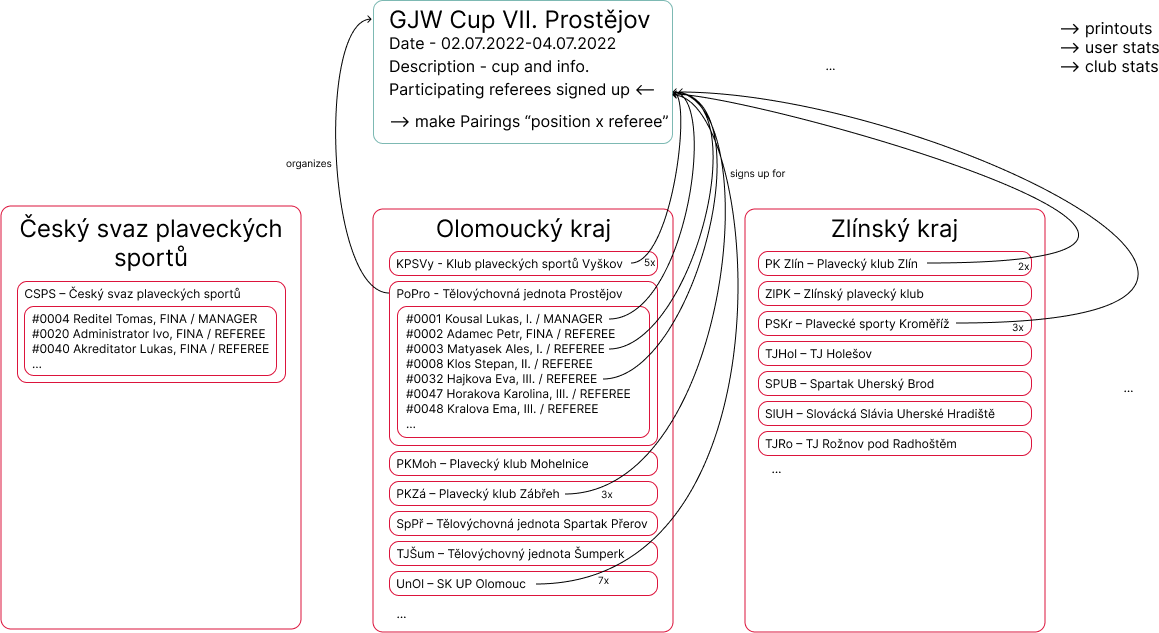
\includegraphics[scale=0.335]{img/swimmpair_schema.png}
\par
The SwimmPair system should deliver public listing of all \textbf{users}, \textbf{cups}, \textbf{news}, \textbf{individual statistics} and \textbf{club statistics}. System should allow to browse stats on a yearly basis. Structure from this image then has to be appropriately modeled with objects. Proposition of database schema will be shown further down. 
%\newpage
\section{Stakeholders}
Groups direclty and indirectly interested in existence of this application and breakdown of its active/passive users.
\subsection*{Interest groups}
There are several entities that are interested in existence of this application. All these stakeholders will have their job facilitated and organized better to some extent thanks to this application.  
Interested stakeholders are:
\begin{itemize}
  \item \textbf{Czech Swimming Federation} - organization for swimming,
  \item \textbf{Olomouc Region}, \textbf{Zlin Region} - regions administered together,
  \item \textbf{Lukas K} - manager who demanded this application.
\end{itemize}
\subsection*{Users of application}
Our users are Czech Swimming Federation members. If their \textbf{region} is \textbf{participating in this application}, clubs and referees from this region must be in our system. With regards to referee's competence level within these clubs, one will have one of these roles: 
\begin{itemize}
  \item \textbf{system administrator} ($\sim$1-3),
  \item \textbf{club manager} + referee ($\sim$10s),
  \item \textbf{referee} ($\sim$100s).
\end{itemize} 
Roles are self-descriptive and previously casually mentioned. My friend, who came up with this idea is \textbf{system administrator} because he's been running all this agenda offline. Club managers are taking care of competitions on behalf of the club and referees are common people who have some degree of knowledge about competitions. Colected statistics will then be used for accreditation granting, activity monitoring and categorization overall.
\par
We were iterating form and features of the web application with two future system administrators during time of development. We then tested usability on all three groups of users via. SUS \footnote{\textbf{System Usability Scale} is a questionnaire to reveal how friendly tested system is to target audience. We carried on initial testing for 20 people belonging to one of these 3 categories to find out if we met at least an average score which was determined to be 68/100.} questionnaire.
%%%An~example citation: %\cite{Andel07}
\section{Functional requirements}
These are the tasks that have to be performed within in our application:
\begin{itemize}
    \item \lbrack club manager\rbrack \,needs to\, \lbrack create swimming cup\rbrack \,in order to\, \lbrack publish cup and invite others to participate\rbrack,
    \item \lbrack club manager\rbrack \,needs to\, \lbrack create pairing for swimming cup\rbrack \,in order to\, \lbrack finalize preparations of cup the day before it takes place\rbrack,
    \item \lbrack club manager\rbrack \,needs to\, \lbrack manage swimming club\rbrack \,in order to\, \lbrack keep information and users up-to-date\rbrack,
    \item \lbrack club manager\rbrack \,needs to\, \lbrack preview cup and print pairing\rbrack \,in order to\, \lbrack perform inspection and publish information offline\rbrack,
    \item \lbrack club manager\rbrack \,needs to\, \lbrack participate in cup or participate with teammates\rbrack \, in order to\, \lbrack help with swimming cup to happen\rbrack,
    \item \lbrack stakeholder\rbrack \,needs to\, \lbrack have information about participations\rbrack \, in order to\, \lbrack grant accreditations to referees\rbrack,
    \item \lbrack referee\rbrack \,needs to\, \lbrack view statistics of referees\rbrack \, in order to \, \lbrack have track record about participation\rbrack,
    \item \lbrack club manager\rbrack \,needs to\, \lbrack view statistics of clubs\rbrack \, in order to \, \lbrack have information about performance of own club\rbrack,
    \item \lbrack club manager\rbrack \,needs to\, \lbrack perform referees managment\rbrack \, in order to \, \lbrack keep referees up-to-date\rbrack,
    \item \lbrack club manager\rbrack \,needs to\, \lbrack perform club managment\rbrack \, in order to \, \lbrack keep own club up-to-date\rbrack,
    \item \lbrack system administrator\rbrack \,needs to\, \lbrack have overview of clubs\rbrack \, in order to \, \lbrack be informed about happenings (within application)\rbrack,
    \item \lbrack system administrator\rbrack \,needs to\, \lbrack manage referees\rbrack \, in order to \, \lbrack add, remove, update users in the application\rbrack,
    \item \lbrack system administrator\rbrack \,needs to\, \lbrack list referees overview\rbrack \, in order to \, \lbrack see activity of referees\rbrack,
    \item \lbrack system administrator\rbrack \,needs to\, \lbrack publish news\rbrack \, in order to \, \lbrack notify everybody about new things\rbrack,
    \item \lbrack stakeholder\rbrack \,needs to\, \lbrack have overall categorization of federation\rbrack \, in order to \, \lbrack use system for administrative purposes\rbrack,
    \item \lbrack stakeholder\rbrack \,needs to\, \lbrack have database archivation of federation\rbrack \, in order to \, \lbrack use system as archivation tool\rbrack.
    %\item \lbrack SOMEBODY\rbrack \, needs to \, \lbrack TO DO SOMETHING\rbrack \, in order to \, \lbrack SOMETHING\rbrack,
  \end{itemize}
\section{Domain model}
Let's go through things that have to be represented in this system one by one starting from the most important ones. We will outlay  objects, their relations and their relational connections. After that basic idea of entities and their relations will be established we continue to project specification for further implementation. We, however, worked more iteratively so this is just retrospective model for implementation that we were specifying during the time of development. 
\par
\subsection*{Cup}
\textbf{Cup is the most important object of SwimmPair.} A swimming Cup contains name, description, date and is affiliated to organizing Club. Cup serves two purposes. \textbf{Firstly} - assigning referees for specific tasks (time tracking, computer support, head of the cup, etc.) has to be \textbf{ready by the time the event takes place}. \textbf{Secondly} - statistics summing up participations for Users and Clubs have to be calculated for each year over all cups in this time period. We also have to discriminate between upcoming and already past cups. Upcoming cups are displayed on the top, past cups should reside in the archive to be revisited for statistical purposes.
\subsection*{User}
\par
User is an entity modelling swimming referee. A referee participating in this system falls in one of three categories. These categories or levels if you wish are \textbf{referee}, \textbf{club manager} and \textbf{system administrator}. User has to be uniquely identifiable. A person i.e. User in the system is going to have profile information such as first name, family name, email address. Good practice of using email address as a login information is going to be used here. User must also contain SwimmPair hierarchy listed above\footnote{\textbf{Rights} - referee 0 / club manager 1 / system administrator 2} and indicator of one's skill and knowledge in the swimming field\footnote{\textbf{Referee Rank} - 1/2/3/4/FINA - \url{https://www.czechswimming.cz/index.php/rozhodci}}, i.e. referee category. User must also belong to exactly one club in our system.
\subsection*{Club}
\par
Club is an administrative unit grouping people (in the same city). Club has a specific name, abbrevation and ID in Czech Referee Federation. An image can be included as well. A club will be serving as a formal authority organising Cup by a User who is club manager. Club is unanimously affiliated to Region. Statistics regarding performance of members of Club at swimming competitions must be implemented. Statistics have informative characted and will save time in the current status quo - keeping track of presence and work descriptions in Excel spreadsheets.
\subsection*{Region}
One of the 13 regions of the Czech Republic in which this system is used. Clubs are located in one of these regions. When new Club starts using SwimmPair, new region has to be added and potential clubs created and attached to this Region. 
We list objects of our application model and describe their properties and purpose. 
%\subsection*{Post}
%Informative news snippet displayed on the homepage.
%\newpage
\subsection*{Schema mockup}
Majority of focus should be on tables \textbf{users} and \textbf{cups} in presented schema. Users belong to clubs that belong to regions. These two entities \textbf{user} and \textbf{cups} will then be brought together into table called \textbf{availability} which contains referees that are available for specific cups. Availabile users for cup are then paired in \textbf{pairing} where each record can be assigned a position from prescripted \textbf{positions}.
\newline
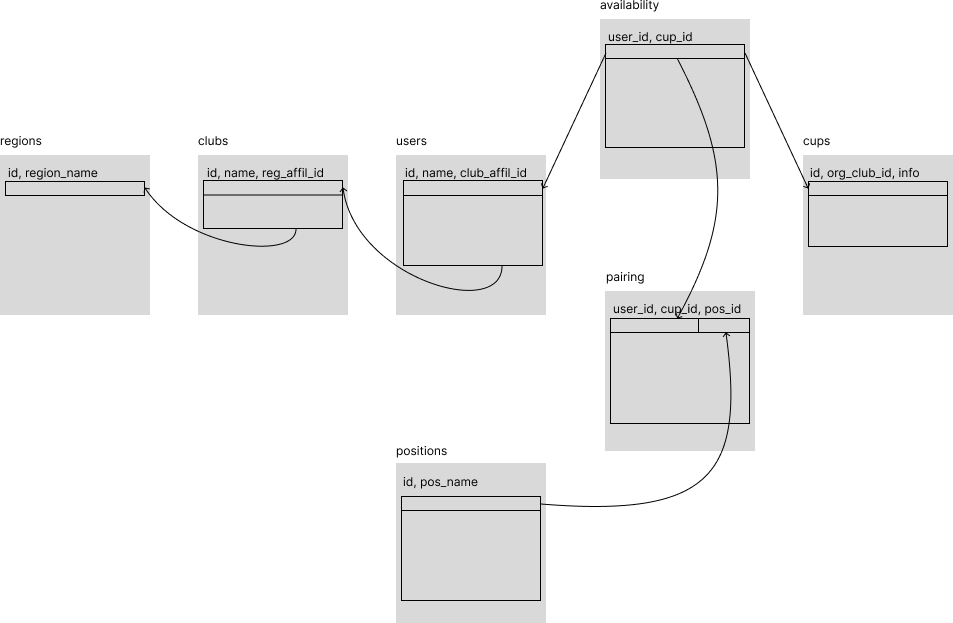
\includegraphics[scale=0.430]{img/swimmpair_db_mockup.png}
\subsection*{Availability}
Takes track of \textbf{User} to \textbf{Cup} availability of who is signed either by their team manager or themselves for the cup. Availability has extra flag going - in case User is paired but can't suddenly go then flag is switched to zero, in order to keep him in pairing but mark him as not going.
\subsection*{Pairing}
Record from \textbf{Availability} is then taken and \textbf{Positions} is assigned to it. 
\subsection*{Position}
Predefined list of tasks necessary to be done at each cup. This list is probably never going to change since there is a fixed set of roles. Referees are going to be assigned to these positions for each cup by drag'n'drop user interface in administration.
\newpage
\section{Quality/Usability requirements}
Several good practices have to be implemented to make SwimmPair easy to use. These practices are either well known or situation specific but they have one thing in common - they should make the application good to use.
\subsection*{Smooth frontend browsing}
\par
Frontend of SwimmPair should be easy to use. There are several options and use cases of JavaScript that can come in handy. Reduction of page reloads is definitely a good way to go. Therefore there are going to be asynchronous JavaScript calls for obtain semi-partial data. After, next function will modify the DOM based on data received from asynchronous call. 
\subsection*{Multiple device types}
\par
Today is certain that there are users who want to browse our system from pc, tablet or smartphone and responsive design is a necessity. Since CSS3 supports media queries\footnote{\url{https://developer.mozilla.org/en-US/docs/Web/CSS/Media_Queries}} we are going to use them for creation of device specific styling.
\subsection*{Assigning referees to positions via. drag'n'drop}
\par
Assigning referees to positions for cups should be implemented via drag'n'drop. Dragging a referee, moving referee over the region specified for the positions and releasing mouse button. Double clicking this person is a good way of removing it.
\subsection*{Printouts of pairing}
Upcoming Cup can be directly printed\footnote{\url{https://developer.mozilla.org/en-US/docs/Web/CSS/Media_Queries/Using_media_queries\#targeting_media_types}} from website and hanged as data printout. 
%\subsection*{Mobile administration}
%Since some things could be done from phone, a phone app without a necessity of web browser will have more native feel. Assigning by drag and drop would be very %hazardeous to do with regards to difference between mouse and finger. Also we are not certain that the Events are the same. Therefore full version %adminsitrative app should be necessary to be provided.
\subsection*{Appropriate design}
\par
Red blue and grey are colors that appear pretty much at a swimming pools. These colors will be used in our system as well. The elements should have fresh lightweave look and not appear heavy.

\chapter{System design}
Reader will be familiarized with architecture of our application. There are two logical parts, \textbf{public web} and \textbf{private administration}. Private administration is hidden behing \textbf{login/password}. 
\par
When designing such system, object oriented approach and grouping of similar functions together is a must. There are objects that have to be moved around the web application described in previous chapter. These objects are Post, User, Club, Cup, Position and Region. Therefore we came up with a concept of managers. Each page of SwimmPair is composed of same headerer, menu, footer. The content part is filled with page's specific results of manager call used to construct data UI page layout. These managers are included and used in all pages via \textbf{start file}.
\section{Technologies}
Following technologies are used to implement SwimmPair application:
\begin{itemize}
    \item \textbf{HTML} is HyperText Markup Language \footnote{\citep{HTML5Standard}} - application pages are templated in HTML by PHP,
    \item \textbf{CSS} is Cascading Style Sheets \footnote{\citep{CSS3Standard}},
    \item \textbf{PHP} is a general-purpose scripting language geared toward web development \footnote{\citep{PHP74Standard}} - object model and backend services are provided by it,
    \item \textbf{JavaScript}  is a general-purpose scripting language that conforms to the ECMAScript specification \footnote{\citep{ECMADocu}},
    \item \textbf{MySQL} is an open-source relational database management system \footnote{\citep{MySQLDocu}},
    \item \textbf{Git} is a distributed version control system: tracking changes in any set of files - this project is versioned and kept in public GitHub repository \footnote{\url{https://github.com/KlosStepan/SwimmPair-Www}},
    \item \textbf{Docker} is a set of platform as a service products that use OS-level virtualization to deliver software in packages called containers \footnote{\citep{DockerDocu}} - used for deployment of out application,
    \item \textbf{Kubernetes} is an open-source container orchestration system for automating software deployment, scaling, and management \footnote{\citep{K8sDocu}} - used for production deployment of our application into cluster.
\end{itemize} 
\newpage
\section{Architecture overview}
Visitor comes to \textbf{app page}, where \textbf{managers} are included. From page there are API calls on Managers that retrieve and store data data as follows.
\newline
\begin{figure}[h]	
	\centering	
    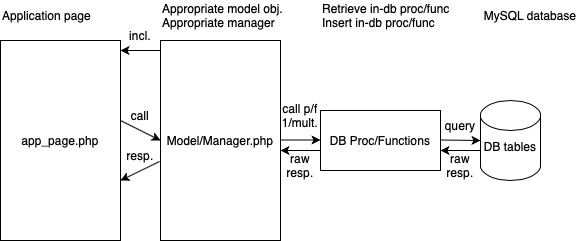
\includegraphics[scale=0.707]{img/app-schema.jpg}
	\caption{From page to manager, database, function, database and back.}
	\label{fig2.1:appschema}
\end{figure}
\section{Model Managers}
Managers are written to provide API functionality for system administration. These managers are populating pages or taking new input from them and administer process of storing them. Each object has a manager handling it and accomodates database loads and stores controlled by transactions.
\begin{itemize}
    \item Cup / CupsManager
    \item User / UsersManager
    \item Club / ClubsManager
    \item Page / PagesManager
    \item Post / PostsManager
    \item Position / PositionsManager
    \item Region / RegionsManager
\end{itemize}
Managers are implemented to extract and store data of class by which they are named after.
\newpage
\section{User Interface mockups}
In this chapter we present UI mockups of some public and private parts of our applicaton. They serve as an initial visualization mockups based on which the real UI will be made. These mockups are not 1:1 guidance, rather an idea for reader and stakeholders for the beginning.  
\subsection*{Public website mockups}
This part is concerned about displaying view-only data for public access.
\begin{figure}[h]	
	\centering	
    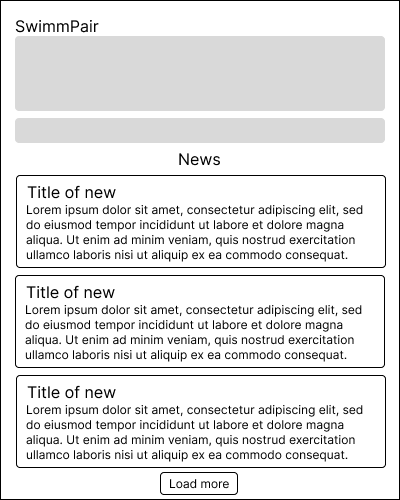
\includegraphics[scale=0.457]{img/def-U-Main.png}
    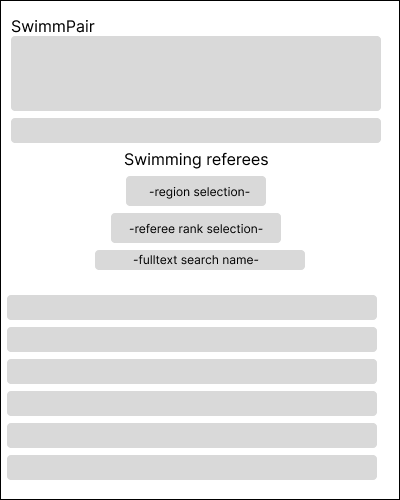
\includegraphics[scale=0.457]{img/def-U-ListingUsers.png}
    %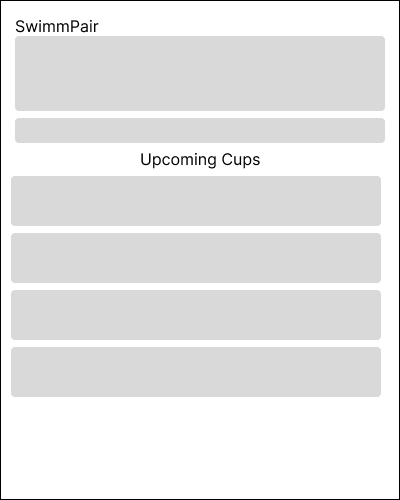
\includegraphics[scale=0.507]{img/def-U-ListingCups.png}
    %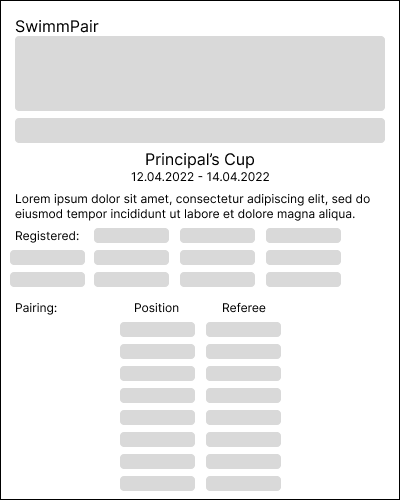
\includegraphics[scale=0.507]{img/def-U-Cup.png}
	\caption{Public pages - \underline{homepage (S5)} and \underline{listing of users (R3/S4)}.}
	\label{fig1.2:fepublicpages1}
\end{figure}
\begin{figure}[h]	
	\centering	
    %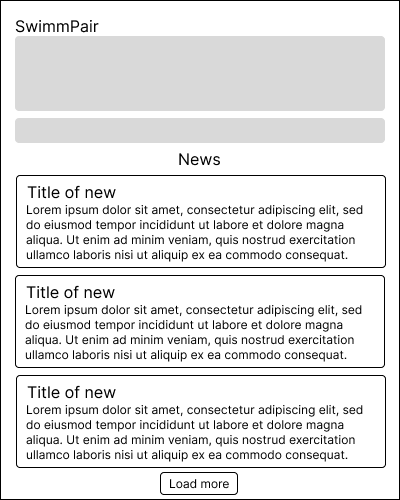
\includegraphics[scale=0.507]{img/def-U-Main.png}
    %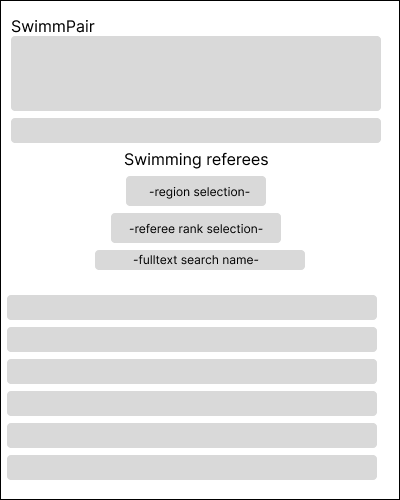
\includegraphics[scale=0.507]{img/def-U-ListingUsers.png}
    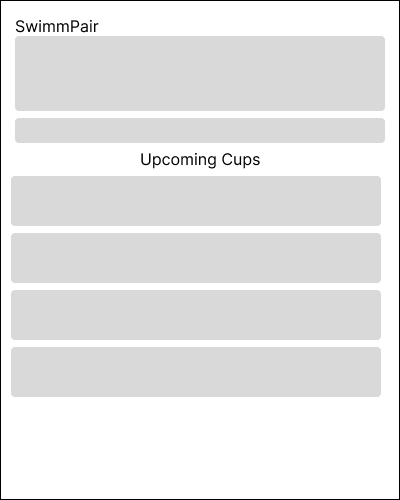
\includegraphics[scale=0.457]{img/def-U-ListingCups.png}
    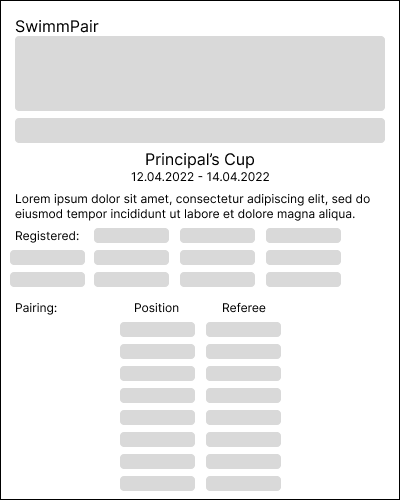
\includegraphics[scale=0.457]{img/def-U-Cup.png}
	\caption{Public pages - \underline{cups listing and cup preview (C3)}.}
	\label{fig1.3:fepublicpages2}
\end{figure}
%\newline
%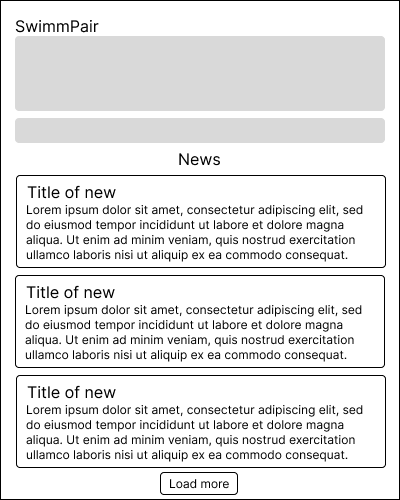
\includegraphics[scale=0.507]{img/def-U-Main.png}
%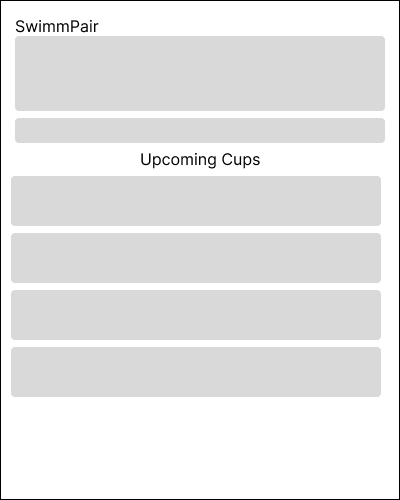
\includegraphics[scale=0.507]{img/def-U-ListingCups.png}
%\newline
%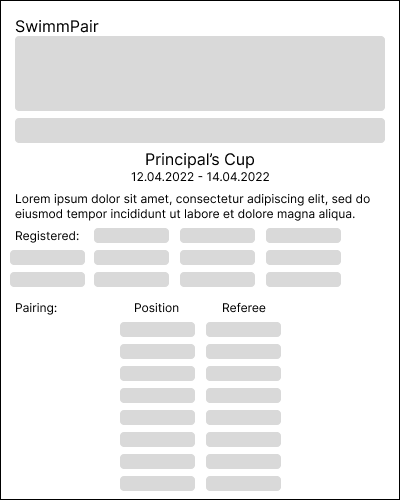
\includegraphics[scale=0.507]{img/def-U-Cup.png}
%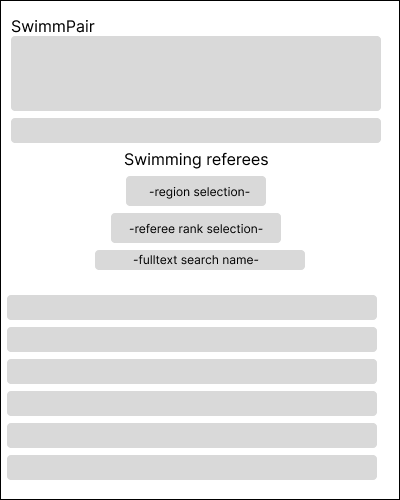
\includegraphics[scale=0.507]{img/def-U-ListingUsers.png}
\newpage
\subsection*{Administration mockups}
After logging in, user can see administrative menu. Based on rights (2/1/0) one gets layout of  appropriate sections. There is list things related to everything from administrative perspective. We will show several mockups of how functional requirements for administration can look like once programmed and designed. 
\begin{figure}[h]	
	\centering	
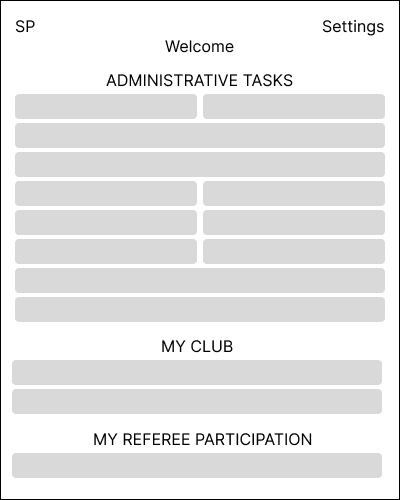
\includegraphics[scale=0.457]{img/A-administrace.png}
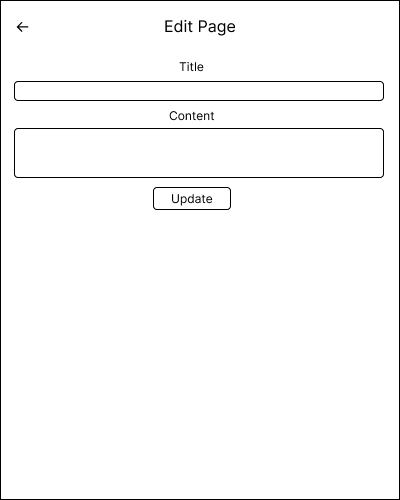
\includegraphics[scale=0.457]{img/A-edit-page.png}
\caption{Administration menu gets assembled on rights, \underline{page edit (S6)}.}
\label{fig1.4:feprivatepages1}
\end{figure}
\begin{figure}[h]	
	\centering
    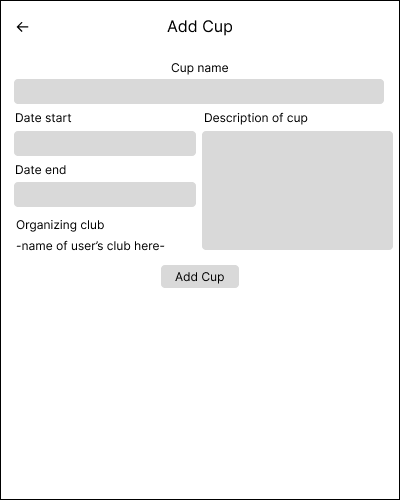
\includegraphics[scale=0.457]{img/A-new-cup.png}
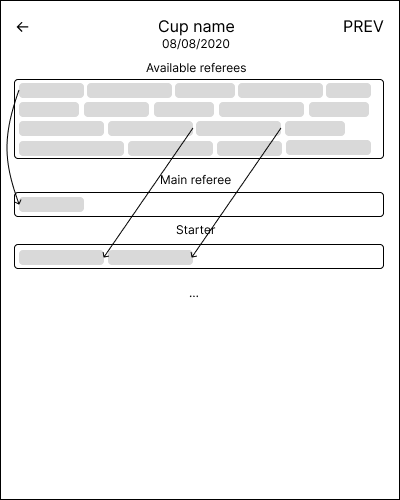
\includegraphics[scale=0.457]{img/A-pairing.png}
\caption{\underline{Add Cup (C1)} and \underline{drag'n'drop pairing (C2)}.}
\label{fig1.5:feprivatepages2}
\end{figure}
\newpage
\section{Database design}
While designing such, system a well defined database schema modelled on functional requirements is a necessity. Previously outlied real world (\autoref{fig1.2:uml}) has to be rigorously converted to database schema.
\iffalse
We will show basic database schema, which should be understandable after knowledge of UML schema (\autoref{fig1.2:uml}).  
\newline
\textbf{Basic preview schema}
\begin{figure}[h]	
    \centering	
    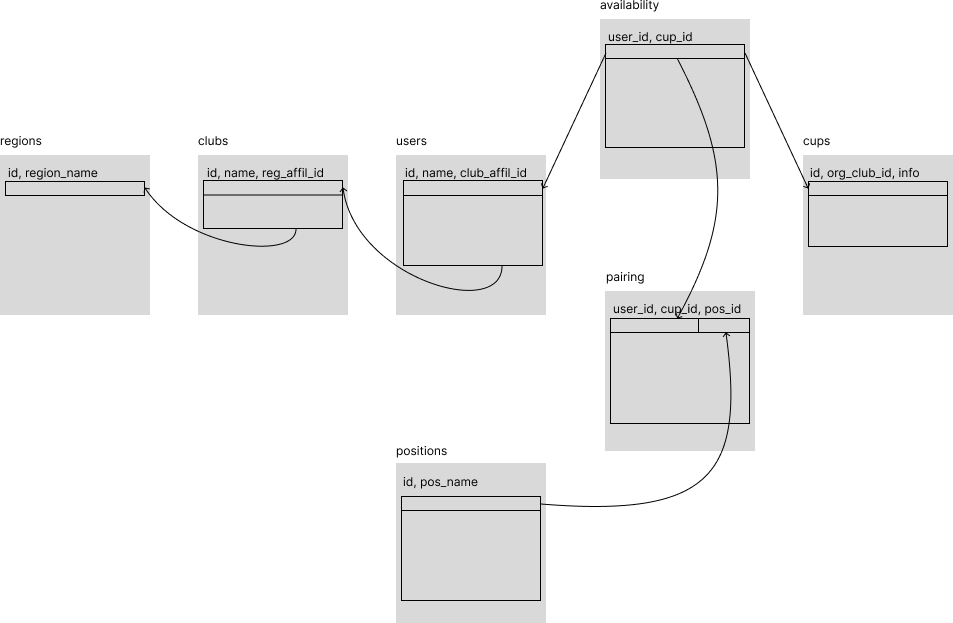
\includegraphics[scale=0.33]{img/swimmpair_db_mockup.png}
    \caption{Simplified schema without all information just for idea.}
    \label{fig2.6:dbschemasimpl}
\end{figure}
\newline
\fi

\textbf{Full database schema used for out application}
\begin{figure}[h]	
	\centering	
    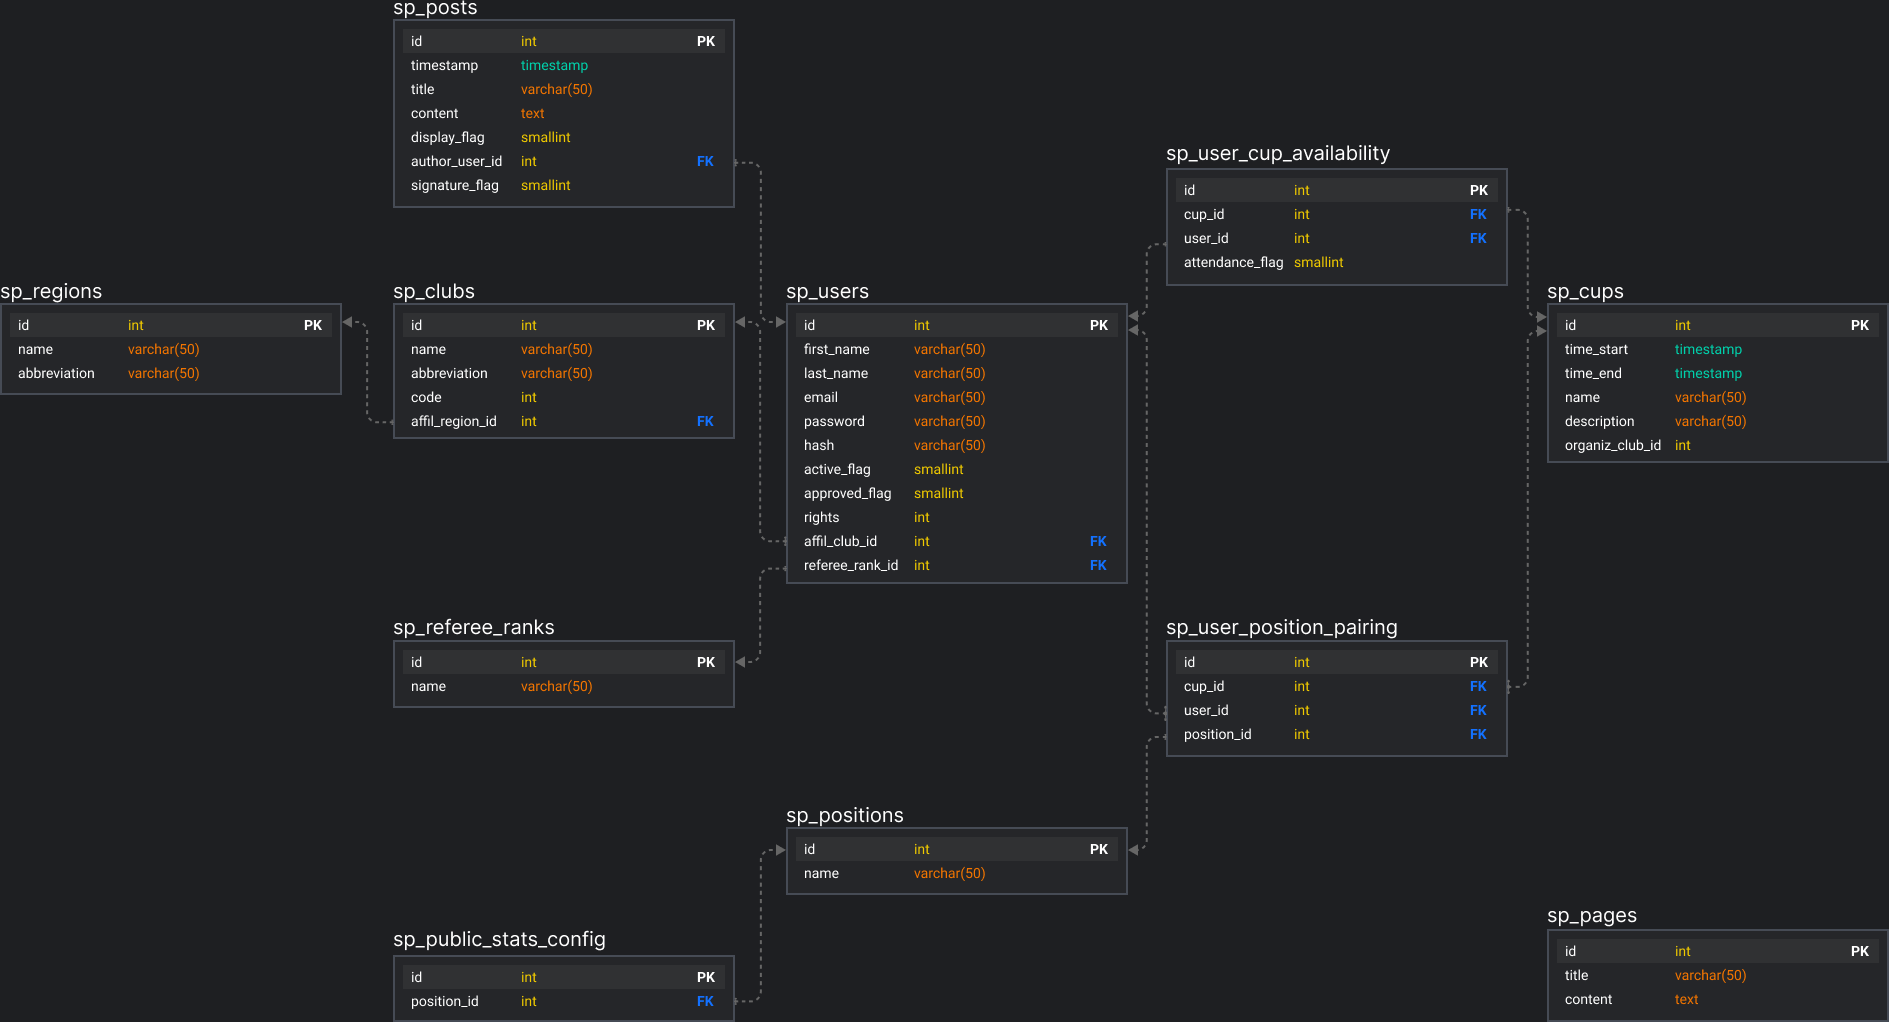
\includegraphics[scale=0.2175]{img/swimmpair_db_schema.png}
	\caption{Full database schema for the SwimmPair application.}
	\label{fig2.7:dbschemafull}
\end{figure}

\iffalse
% Let's take PostsManager as an example. This manager handles Post and is implemented as follows.
\textbf{Object - Post.php}
\begin{lstlisting}
class Post
{
    public $id;
    public $timestamp;
    public $title;
    public $content;
    public $display_flag;
    public $author_user_id;
	public $signature_flag;

    public function __construct($id, $timestamp, $title, $content, $display_flag, $author_user_id, $signature_flag)

	//7/7: {id, timestamp, title, content, display_flag, author_user_id, signature_flag}
	public function Serialize()
}

\end{lstlisting}
\textbf{Manager - PostsManager.php} 
\begin{lstlisting}
class PostsManager
{
	private $mysqli;

    //Constructor - setting $mysqli to $this->mysqli
	public function __construct(mysqli $mysqli)

    //Handling functions retrieve/store  
	public function GetPostById($id)
  	public function FindLastNPosts($N)
	public function InsertNewPost($title, $content, $display_flag, $author, $signature_flag)
    public function UpdatePost($id, $title, $content, $display_flag, $signature_flag)

    //Private functions - auxiliary controller functions
	private function _CreatePostOrNullFromStatement(mysqli_stmt $statement)
	private function _CreatePostsFromStatement(mysqli_stmt $statement)
	private function _CreatePostFromRow(array $row)
}
\end{lstlisting}
\textbf{Demonstration - public function GetPostById(\$id)}
\begin{lstlisting}
public function GetPostByID($id)
{
	$statement = $this->mysqli->prepare("CALL `GetPostById`(?);");
	$statement->bind_param('i', $id);
	return $this->_CreatePostOrNullFromStatement($statement);
}
\end{lstlisting}
Objects and their managers are made in the same manner. They contain different set of data and different number public functions. Description is included in documentation chapter below. 
\fi
\iffalse
\section{Responsive layout}
Listed media queries are used to provide design of the web by manually overriding specific classes for desired user experience outcome.
\begin{itemize}
    \item Basic CSS design
    \item @media (max-width: 768px)
    \item @media (print)
\end{itemize}
\textbf{Basic CSS design} gives definition of colors and desktop layout of our application. \textbf{Media query with max-width: 768px} supports tablets and mobile devices while \textbf{media print} of cup pairing hides redundant controll and informative elements while it keeps the pairing of cup to be printed.
\fi
\iffalse
\section{Administrative tasks}
\begin{itemize}
    \item \textbf{Add Post/Edit Post} - from PostsManager call \newline InsertNewPost/UpdatePost
    \item \textbf{Approve Newly Registered Users} - swap flag \textbf{approved} to \textbf{1}
    \item \textbf{Pair Available Users On Cup Positions} - from UsersManager call UpdatePairing - calls several SQL Procs for different things in transaction and commits/rollbacks
    \item \textbf{Add User/Edit User} - from UsersManager call AddUser/UpdateUser
    \item \textbf{Add Cup/Edit Cup} - from CupsManager call AddCup/UpdateCup
    \item \textbf{Add Club/Edit Club} - from ClubsManager call AddClub/UpdateClub
    \item \textbf{Add Region/Edit Region} - from RegionsManager call AddRegion/UpdateRegion
    \item \textbf{Configure Stats Ordering} - delete ordering, insert ordering \textbf{Nth}-\textbf{statId} 
    \item \textbf{Edit Contacts} - from PagesManager call UpdatePage
\end{itemize} 
\section{Club Manager tasks}
\begin{itemize}
    \item \textbf{Add Cup} - from CupsManager call AddCup
    \item \textbf{Sign Up People From My Club As Available For Cup} - prihlasit\_moje\_lidi\_na.php then XMLHttpRequest/call\_update\_availability.php
\end{itemize}   
\section{Referee tasks}    
\begin{itemize}
    \item \textbf{Sign Myself As Available For Cup} - add my Id to table \textbf{cupId}-\textbf{userId}
\end{itemize}
\fi
\newpage
\section {Functional requirements mapping to API}
We will show how specific \textbf{functional requirements} administrative tasks are realized via \textbf{model api functions}\footnote{\url{http://docu.swimmpair.cz/functions_func.html}}.
\newline
Table has following structure: \textbf{Task} / \textbf{Role} / \textbf{Function(s)}.
\newline
\begin{tabularx}{1.0\textwidth} { 
  | >{\raggedright\arraybackslash}X 
  | >{\centering\arraybackslash}X 
  | >{\raggedright\arraybackslash}X | }
 \hline
 Add Post & system admin& InsertNewPost \\
 \hline
 Edit Post  & system admin  & UpdatePost \\
 \hline
 Approve New Users & system admin & SetApprovedForUser \\
 \hline
 Create Pairing For Cup & system admin & DeleteOldPairing
InsertNewPairing\\
 \hline
 Add User & system admin & RegisterUser \\
 \hline
 Edit User & system admin &
 SetLoginEmailForUser
 SetRefereeRankForUser
 SetPasswordForUser\\
 \hline
 Add Club & system admin & InsertNewClub \\
 \hline
 Edit Club & system admin & UpdateClub \\
 \hline
 Add Region & system admin & InsertNewRegion \\
 \hline
 Edit Region & system admin & UpdateRegion \\
 \hline
 Configure Stats & system admin & DeleteOldStatsPositions
 InsertNewStatPosition \\
 \hline
 Edit Contacts & system admin & UpdatePage \\
 \hline
 Add Cup & club manager & InsertNewCup \\
 \hline
 Sign People From My Club Available For Cup & club manager & DeleteOldAvailability
 InsertNewAvailability \\
 \hline
 Sign Myself As Available For Cup & referee & SetAvailabilityRegister
 SetAvailabilityCantGo 
 SetAvailabilityCanGo \\
\hline
\end{tabularx}
\iffalse
These functions are used for \underline{retrieving} data to navigate across the administration.
\begin{itemize}
    \item Posts: FindAllPostsOrderByIDDesc
    \item Approve Users: FindAllInactiveUsersOrderByLastNameAsc
    \item Cups For Pairings: FindAllUpcomingCupsEarliestFirst
    \item Users: FindAllUsers
    \item Clubs: FindAllClubs
    \item Regions: FindAllRegions
    \item Stats: FindAllPositions, DisplayedLiveStatsConfiguredPositions
    \item Pages: GetPageByID
    \item Sign People From My Club Available For Cup : FindAllUpcomingCupsEarliestFirst, GetCupByID, FindAllTeamMembers, FindAllRegisteredTeamMembersForTheCup
    \item Sign Myself As Available For Cup: FindAllUpcomingCupsEarliestFirst, GetCupByID, IsUserAvailableForTheCup, IsComing
\end{itemize}
\fi
\chapter{Implementation}
DDetailed description of all components and  functions here.  
\begin{csharpcode}
//UDPHandler Constructor 
public UDPHandler(String IP, Int32 Port, Int32 Timeout)
{
    ServerAddr = IPAddress.Parse(IP);
    EndPoint = new IPEndPoint(ServerAddr, Port);
    sock.ReceiveTimeout = Timeout;
    s = new UdpClient(IP, Port);
    
    EncryptionKeyDefault = "YiyM/f2zNq5GkVmiUMJ8qVACaPaBBo5AJRqkIH9cgd4=";
    EncryptionIVDefault = "tLafaj6+1YCiIIvbMO7iN/9QVLK1PPjRzARR9Fsh82c=";
}
\end{csharpcode}
PHP Code
\begin{phpcode}
<?php
class Payload
{
    public $Nth;
    public $outOfN;
    public $content;
    //konstruktor
    public function __construct($Nth, $outOfN, $content)
    {
        $this->Nth = $Nth;
        $this->outOfN = $outOfN;
        $this->content = $content;
    }
}
?>
\end{phpcode}

\section{Database design}
dbd
\subsection{Object tables}
\subsection{Relationship tables}
\subsection{Schema}
Export a picture here.
\section{Controllers documentation}
\par These five controllers are used followingly
\subsection{PostsManager.php}
\begin{itemize}
  \setlength\itemsep{0em}
  \item \underline{Post} $\vert$ null $\leftarrow$ \textbf{GetPostById}(\$id) $\searrow$ \_CreatePostOrNullFromStatement(\$stmt) $\searrow$ \_CreatePostFromRow(\$row)
  \item \underline{Post[]} $\vert$ null $\leftarrow$ \textbf{GetLastThreePosts}() $\searrow$ \_CreatePostsFromStatement() $\searrow$ \_CreatePostFromRow(\$row)
  \item \underline{Post[]} $\vert$ null $\leftarrow$ \textbf{GetLastNPosts}(\$N) $\searrow$ \_CreatePostsFromStatement() $\searrow$ \_CreatePostFromRow(\$row)
  \item \underline{true} $\vert$ false $\leftarrow$ \textbf{AddNewPost}(\$title, \$content)
  \item \underline{Post[]} $\vert$ false $\leftarrow$ \textbf{FindAllPostsOrderedByIdDesc}() $\searrow$ \_CreatePostsFromStatement(\$stmt) $\searrow$ \_CreatePostFromRow(\$row)
  \item \underline{true} $\vert$ false $\leftarrow$ \textbf{UpdatePost}(\$id, \$title, \$article)
\end{itemize}
\subsection{UsersManager.php}
\begin{itemize}
  \setlength\itemsep{0em}
  \item \underline{User} $\vert$ null $\leftarrow$ \textbf{GetUserById}(\$id) $\searrow$ \_CreateUserOrNullFromStatement(\$stmt) $\searrow$ \_CreateUserFromRow(\$row)
  \item \underline{User[]} $\vert$ null $\leftarrow$ \textbf{FindAllActiveUsersOrderByLastNameDesc} $\searrow$ \_CreateUsersFromStatement(\$stmt) $\hookrightarrow$ \_CreateUserFromRow (\$row)
  \item \underline{User[]} $\vert$ null $\leftarrow$ \textbf{FindAllInactiveUsersOrderByLastNameDesc} $\searrow$ \_CreateUsersFromStatement(\$stmt) $\hookrightarrow$ \_CreateUserFromRow (\$row)
  \item \underline{User[]} $\vert$ null $\leftarrow$ \textbf{FindAllRegisteredComradesForTheCup}(\$cupID, \$teamID) $\searrow$ \_CreateUsersFromStatement(\$stmt) $\hookrightarrow$ \_CreateUserFromRow (\$row)
  \item \underline{User[]} $\vert$ null $\leftarrow$ \textbf{FindAllComrades}(\$teamID) $\searrow$ \_CreateUsersFromStatement(\$stmt) $\hookrightarrow$ \_CreateUserFromRow(\$row)
  \item \underline{User[]} $\vert$ null $\leftarrow$ \textbf{FindAllRegisteredUsersForTheCup}(\$cupID) $\searrow$ \_CreateUsersFromStatement(\$stmt) $\hookrightarrow$ \_CreateUserFromRow(\$row)
  \item \underline{User[]} $\vert$ null $\leftarrow$ \textbf{FindAllNametagsForTheCup}(\$cupID) $\searrow$ \_CreateUsersFromStatement(\$stmt) $\hookrightarrow$ \_CreateUserFromRow(\$row)
  \item \underline{User[]} $\vert$ null $\leftarrow$ \textbf{FindPairedUsersOnCupForPosition}(\$cupID, \$posID) $\searrow$ \_CreateUsersFromStatement(\$stmt) $\hookrightarrow$ \_CreateUserFromRow(\$row)
  \item \underline{Pair[]} $\vert$ null $\leftarrow$ \textbf{FindPairedPozIDUserIDOnCup}(\$cupID) $\searrow$ \_CreatePairsFromStatement(\$stmt) $\hookrightarrow$ \_CreatePairFromRow(\$row)
  \item \underline{string} $\vert$ null $\leftarrow$ \textbf{GetClubAbbreviationByAffiliationId}(\$id) $\searrow$ \_GetSingleResultFromStatement(\$stmt)
  \item \underline{string} $\vert$ null $\leftarrow$ \textbf{GetUserFullNameById}(\$id) $\searrow$ \_GetSingleResultFromTwoColsStatement(\$stmt)
  \item \underline{true} $\vert$ \underline{false} $\leftarrow$ \textbf{UserWithEmailExists}(\$email)
  \item \underline{true} $\vert$ false $\leftarrow$ \textbf{RegisterUserFromAdmin}(\$first\_name, \$last\_name, \$email, \$password, \$rights, \$klubaffil)
  \item \underline{true} $\vert$ false $\leftarrow$ \textbf{SendYouWereRegisteredFromAdmin}(\$email, \$password)
  \item \underline{true} $\vert$ false $\leftarrow$ \textbf{ApproveUser}(\$userID)
  \item \underline{true} $\vert$ false $\leftarrow$ \textbf{UpdatePairing}(\$JSON) //TBReimplemented in controller
  \item \underline{true} $\vert$ false $\leftarrow$ \textbf{RegisterUserFromAdminWrap}(\$first\_name, \$last\_name, \$email, \$password, \$prava, \$klub) check, register if possible ($\searrow$ true(not registering) | \underline{false} $\leftarrow$ userWithEmailExists(\$email) | $\searrow$ registerUserFromAdmin(\$first\_name, \$last\_name, \$email, \$password, \$prava, \$klub))
  \item \underline{token(Action::SUCC, -creds-)} $\vert$ token(Action::UNFOUND, -null-) | token(Action::WRONGCRED, -null-) $\leftarrow$ \textbf{loginFromXamarin}(\$username, \$password)
\end{itemize}
\subsection{ClubsManager.php}
\begin{itemize}
  \setlength\itemsep{0em}
  \item \underline{Club} | null $\leftarrow$ \textbf{GetClubById}(\$id) $\searrow$ \_CreateClubFromStatement(\$stmt) $\searrow$ \_CreateClubFromRow(\$row)
  \item \underline{Club []} | null $\leftarrow$ \textbf{FindAllClubs}() $\searrow$ \_CreateClubsFromStatement(\$stmt) $\hookrightarrow$ \_CsreateClubFromRow(\$row)
\end{itemize}
\subsection{CupsManager.php}
\begin{itemize}
  \setlength\itemsep{0em}
  \item \underline{Cup[]} $\vert$ null $\leftarrow$ \textbf{FindAllUpcomingCupsEarliestFirst}() $\searrow$ \_CreateCupsFromStatement(\$stmt) $\hookrightarrow$ \_CreateCupFromRow(\$row)
  \item \underline{Cup[]} $\vert$ null $\leftarrow$ \textbf{FindAllPastCupsMostRecentFirst}() $\searrow$ \_CreateCupsFromStatement(\$stmt) $\hookrightarrow$ \_CreateCupFromRow(\$row)
  \item \underline{string} $\vert$ null  $\leftarrow$ \textbf{GetCupNameById}(\$id) $\searrow$ \_GetSingleResultFromStatement(\$stmt) $\searrow$ \_GetSingleResultFromStatement (\$stmt)
  \item \underline{Cup} $\vert$ null  $\leftarrow$  \textbf{GetCupById}(\$id) $\searrow$ \_CreateCupOrNullFromStatement(\$stmt)  $\searrow$ \_CreateCupFromRow(\$row)
  \item \underline{Pair[]} $\vert$ null $\leftarrow$  \textbf{FindPairingsForThisCup}(\$id) $\searrow$ \_CreatePairsFromStatement(\$stmt) $\hookrightarrow$ \_CreatePairFromRow(\$row)
  \item \underline{true} $\vert$ false $\leftarrow$  \textbf{InsertNewCupFromAdmin}(\$name, \$date, \$club, \$content)
  \item \underline{true} $\vert$ \underline{false} $\leftarrow$  \textbf{IsUserAvailableForTheCup}(\$userID, \$cupID)
  \item \underline{true} $\vert$ false $\leftarrow$  \textbf{UpdatePairingForThisCup}(\$cupID, \$json)
  \item \underline{true} $\vert$ false $\leftarrow$  \textbf{UpdateAvailabilityForThisCup}(\$cupID, \$json)
  \item \underline{true} $\vert$ false $\leftarrow$  \textbf{AddAvailableUserForTheCup}(\$cupID, \$userID)
\end{itemize}
\subsection{PositionsManager.php}
\begin{itemize}
  \setlength\itemsep{0em}
  \item \underline{Position[]} $\vert$ null $\leftarrow$  \textbf{FindAllPositions}() $\searrow$ \_CreatePositionsFromStatement(\$stmt) $\hookrightarrow$ \_CreatePositionFromRow(\$row)
  \item \underline{string} $\vert$ null $\leftarrow$ \textbf{GetPositionNameById}(\$id) $\searrow$ \_GetSingleResultFromStatement(\$stmt)
\end{itemize}
\section{Application structure}
\subsection*{User part of the system}
Whole system must be running on Czech URLs for convinience reasons of administrators. English equivalents are attached. 
\newline
\begin{forest}
  for tree={
    font=\ttfamily,
    grow'=0,
    child anchor=west,
    parent anchor=south,
    anchor=west,
    calign=first,
    edge path={
      \noexpand\path [draw, \forestoption{edge}]
      (!u.south west) +(7.5pt,0) |- node[fill,inner sep=1.25pt] {} (.child anchor)\forestoption{edge label};
    },
    before typesetting nodes={
      if n=1
        {insert before={[,phantom]}}
        {}
    },
    fit=band,
    before computing xy={l=15pt},
  }
[SwimmPair
  [Aktuality index.php \char`\~Posts\char`\~]
  [Zavody \char`\~Cups\char`\~
    [nadchazejici.php \char`\~upcoming.php\char`\~
      [zavod.php \char`\~cup.php\char`\~]
    ]
    [archiv.php \char`\~archive.php\char`\~
      [zavod.php \char`\~cup.php\char`\~] 
    ]
  ]
  [Rozhodci \char`\~Referees\char`\~
    [lide.php \char`\~users.php\char`\~
      [clovek.php \char`\~user.php\char`\~]
    ]
    [kluby.php \char`\~clubs.php\char`\~
      [klub.php \char`\~ club.php\char`\~]
    ]
  ]
  [/pravidla/index.php \char`\~/rules/index.php\char`\~]
  [kontakty.php \char`\~contacts.php\char`\~]
  [/admin/index.php]
]
\end{forest}

\subsection*{User part of the system} 
Administration
\begin{itemize}
    \item pridat\textunderscore aktualitu.php - PŘIDAT AKTUALITU 
    \item editovat\textunderscore aktuality.php - EDITOVAT AKTUALITY -\textgreater editovat\textunderscore aktualitu.php
    \item nove\textunderscore registrovani.php - SCHVÁLIT NOVÉ LIDI 
    \item zaregistrovat\textunderscore uzivatele.php - ZAREGISTROVAT ČLOVĚKA
    \item editovat\textunderscore profily.php EDITOVAT ČLOVĚKA -\textgreater editovat\textunderscore profil.php
    \item novy\textunderscore klub.php NOVÝ KLUB
    \item sprava\textunderscore klubu.php - EDITOVAT KLUB -\textgreater editovat\textunderscore klub.php
    \item novy\textunderscore kraj.php PŘIDAT KRAJ
    \item sprava\textunderscore kraju.php SPRÁVA KRAJŮ -\textgreater editovat\textunderscore kraj.php
    \item konfigurace\textunderscore statistik.php - KONFIGURACE STATISTIK
    \item editovat\textunderscore stranku?id=1 - EDITOVAT KONTAKTY
\end{itemize}      
My Club
\begin{itemize}
    \item pridat\textunderscore zavod.php - PŘÍDAT ZÁVOD
    \item prihlasit\textunderscore moje\textunderscore lidi.php - PŘIHLÁÍSIT LIDI Z MÉHO -\textgreater prihlasit\textunderscore moje\textunderscore lidi\textunderscore na.php
\end{itemize} 
Me referee
\begin{itemize}
    \item sebe\textunderscore na\textunderscore zavod.php - PŘIHLÁSIT SE NA ZÁVOD -\textgreater prihlasit\textunderscore se\textunderscore na.php
\end{itemize}    
\section{JavaScript functions documentation}
Several cool features for the web to make it more useful are described here.
\subsection*{XMLHttpRequest/}
\begin{itemize}
    \item getarticleid.php, \textbf{GET args}: id
    \item getpersonstatisticsfortheseason.php, \textbf{GET args}: user\textunderscore id, year
    \item getclubstatisticsfortheseason.php, \textbf{GET args}: club\textunderscore id, year
\end{itemize}
\subsection{Previous post}
This button on the main page serves as a tool for loading next post. This button has onclick="GetPostAppendPost(PushLastID())". These are both JavaScript functions, PushLastID() detects id "I" of last post from DOM by query and returns it. This value is then used as an argument of call GetPostAppendPost(I). This function requests article by opening GET request XMLHttpRequest/getarticleid?id="I". If result is null, button is deleted since there are no other articles to pull from DB. Otherwise next article is constructed.
\subsection{Personal statistics change year}
All individual referees have season picker when opened. Default season is this season. Clicking different season visibily changes selected year and obtains statistics and updates the table. Clicking onclick="processPersonForTheSeason(user-id, updatePairingForThisCup)" calls communicateStatsXHRAndPopulateStats(user-id, year) which gets data from XMLHttpRequest/getpersonstatisticsfortheseason. 
\subsection{Club statistics change year}
Club statistics are updated by clicking appropriate year, which gets visibly switched. Year onclick calls processClubForTheSeason(club-id, this) which gets statistics by calling communicateClubStatisticsXMHAndPopulateTable(club-id, year) which gets data by calling XMLHttpRequest/getclubstatisticsfortheseason and subsequently calling refreshClubStatsInTheTable(returnedGetJSON) which literally puts the stats in.
\subsection{Filtering referees}
This function is triggered by one of these: KrajPickerTapped(this), TridaPickerTapped(this) or SearchPerformed(). Each one calls FilterRozhodci("kraje", "tridy", "inputTrida", "nopplfound"). We then loop all people visible/hidden and check if this one's Region IsPermissible(args[]), then if one's Class IsPermissible(args[]) and then if one's IsNamePermissible(args[]). We then set one element style to style="" and continue cycle execution. If we fail one of these three conditions we proceed to code below which sets element style to style="display:none". After the cycle when check the aux variable and if our query is indeed empty we write it for the user.
\par
This long procedure gets triggered and subsequently executed everytime region, class or name is changed. Performance should be fine here since the algorithm is dependent on human input. 
\section{Mobile app structure}
Phone version of our administration follows the same structure. All objects are same, including data type, which have to be explicitly defined, unline in PHP.
\section{Mobile app communication}

\chapter{Testing}
There are two main ways to make sure that a web application works properly and fulfills its role. On one hand there is a code performance testing, performing test on backend level with dummy data insertion and performance benchmarking. On the other hand there is testing to assure that users are able to use system and to get inspiration for future UX improvements via SUS.
\section{Performance testing}
Performance script \textbf{dummy\_data\_benchmark.php} \footnote{In https://github.com/KlosStepan/SwimmPair-Www \textbf{dummy\_data\_benchmark.php}} is located in main swimmpair folder. It is performed on default database installation (with 2 admin users, with already existing clubs administered by application requesters, and with default referee positions).  
\newline
\textbf{The script has several tasks (tests) which are performed and benchmarked.}
\begin{enumerate}
    \item \underline{Create 98 Users} (no. 3-100) - each random affiliation to existing Club (no. 1-15).
    \item \underline{Create 12 Cups} - each random affiliation to existing Club (no. 1-15).
    \item \underline{Fetch new Users}, \underline{fetch new Cups} (+ \underline{fetch static Positions}).
    \item \underline{Create Availabilities} (20 Users available per Cup).
    \item \underline{Create Pairings} (each Availability gets 1 random position).
    \item \underline{Call stats queries} (20 - randomly either Clubs or Users stats w/ random club\_id or user\_id).
\end{enumerate}
\textbf{Docker Compose} - 2.3 GHz Core i5 (I5-8259U) RAM 16GB Storage 512GB
\newline
\begin{tabular}{ |c|c|c|c|c|c|c|c|c|c|c|c| } 
    \hline
    T/rep no. & \#1 & \#2& \#3& \#4& \#5& \#6& \#7& \#8& \#9& \#10 \\
    \hline
    Test \#1 & 7.02 & 7.04& 6.61& 7.89& 6.73& 6.62& 6.66& 7.34& 7.19& 6.54 \\ 
    Test \#2 & 0.08 & 0.06& 0.06& 0.06& 0.06& 0.10& 0.58& 0.60& 0.50& 0.15 \\ 
    Test \#3 & 7.02 & 7.05& 6.61& 7.90& 6.74& 6.63& 6.66& 7.35& 7.20& 6.55 \\ 
    Test \#4 & 1.24 & 1.05& 1.14& 1.05& 1.18& 1.17& 1.24& 1.15& 0.96& 1.59 \\ 
    Test \#5 & 8.02 & 7.87& 7.39& 8.95& 7.70& 7.81& 7.44& 8.12& 7.98& 7.36 \\ 
    Test \#6 & 1.29 & 1.10& 1.19& 1.12& 1.23& 1.22& 1.28& 1.19& 1.00& 1.62 \\ 
    TOTAL & \underline{9.31} & \underline{8.97}& \underline{8.59}&\underline{10.06}& \underline{8.93}& \underline{9.03}& \underline{8.72}& \underline{9.31}& \underline{8.98}& \underline{8.98} \\ 
    \hline
\end{tabular}
\newline
\textbf{Kubernetes} - \textbf{DOKS} Kubernetes v 1.25.4-do.0, s-1vcpu-2gb-intel
\newline
\begin{tabular}{ |c|c|c|c|c|c|c|c|c|c|c|c| } 
    \hline
    T/rep no. & \#1 & \#2& \#3& \#4& \#5& \#6& \#7& \#8& \#9& \#10 \\
    \hline
    Test \#1 & 7.08 & 6.87& 6.79& 6.85& 7.20& 7.10& 6.77& 6.85& 6.81& 6.79 \\ 
    Test \#2 & 0.04 & 0.03& 0.04& 0.04& 0.04& 0.03& 0.05& 0.05& 0.03& 0.04 \\ 
    Test \#3 & 7.08 & 6.88& 6.79& 6.86& 7.20& 7.10& 6.77& 6.85& 6.81& 6.79 \\ 
    Test \#4 & 0.84 & 0.59& 0.68& 0.81& 0.60& 0.55& 0.70& 0.82& 0.60& 0.67 \\ 
    Test \#5 & 7.72 & 7.40& 7.55& 7.56& 7.69& 7.60& 7.35& 7.56& 7.33& 7.40 \\ 
    Test \#6 & 0.86 & 0.61& 0.70& 0.84& 0.62& 0.57& 0.72& 0.84& 0.62& 0.69 \\ 
    TOTAL & \underline{8.57} & \underline{8.01}& \underline{8.25}& \underline{8.40}& \underline{8.31}& \underline{8.17}& \underline{8.07}& \underline{8.39}& \underline{7.95}& \underline{8.09} \\ 
    \hline
\end{tabular}
\section{User testing}
We carried on testing of our application by handing SUS questionare to 20 respondents. We then evaluated the scores in order to find out how our application stands. These people are are either managers or common referees \footnote{\cite{SUSDesc}}. 
\newline
\textbf{Questionare is made of 10 questions scored 1-5.}
\begin{enumerate}
    \item I think that I would like to use this system frequently.
    \item I found the system unnecessarily complex.
    \item I thought the system was easy to use.
    \item I think that I would need the support of a technical person to be able to use this system.
    \item I found the various functions in this system were well integrated.
    \item I thought there was too much inconsistency in this system.
    \item I would imagine that most people would learn to use this system very quickly.
    \item I found the system very cumbersome to use.
    \item I felt very confident using the system.
    \item I needed to learn a lot of things before I could get going with this system.
\end{enumerate}
\textbf{We calculated\footnote{((A1-1)+(5-A2)+(A3-1)+(5-A4)+(A5-1)+(5-A6)+(A7-1)+(5-A8)+(A9-1)+(5-A10))*2,5} SUS feedbacks based on responses from 20 people.}
\newline
\begin{tabular}{ |c|c|c|c|c|c|c|c|c|c|c|c| } 
    \hline
    Respondent / Q. no. & \#1 & \#2& \#3& \#4& \#5& \#6& \#7& \#8& \#9& \#10 \\
    \hline
    Petr A - \textbf{87.5}     & 5 & 1& 3& 1& 5& 1& 3& 1& 5& 2 \\ 
    Olga A - \textbf{72.5}     & 2 & 1& 3& 2& 4& 1& 5& 1& 3& 3 \\ 
    Marin H - \textbf{75}    & 3 & 1& 4& 2& 5& 1& 3& 2& 3& 2 \\ 
    Michaela H - \textbf{60} & 2 & 3& 3& 4& 3& 2& 4& 2& 5& 2 \\ 
    Stepan K - \textbf{85}   & 5 & 2& 4& 1& 3& 1& 3& 1& 5& 1 \\ 
    Matylda K - \textbf{80}  & 4 & 1& 4& 2& 4& 1& 4& 2& 4& 2 \\ 
    Lukas Kour. - \textbf{67.5} & 2 & 2& 5& 2& 4& 1& 4& 2& 2& 3 \\ 
    Jana K - \textbf{60}    & 1 & 2& 3& 2& 5& 2& 3& 2& 2& 2 \\ 
    Lukas Kous. - \textbf{92.5} & 5 & 1& 4& 1& 5& 1& 4& 1& 5& 2 \\ 
    Zuzana K - \textbf{70}   & 3 & 2& 5& 1& 3& 1& 3& 2& 3& 3 \\ 
    Eva K - \textbf{80}      & 3 & 2& 5& 1& 3& 1& 3& 1& 4& 1 \\ 
    Michael P - \textbf{75}  & 2 & 1& 4& 3& 4& 1& 4& 1& 3& 1 \\ 
    Lenka P - \textbf{70}    & 3 & 2& 5& 1& 3& 2& 3& 2& 3& 2 \\ 
    Daniela S - \textbf{77.5}  & 3 & 2& 5& 2& 3& 1& 4& 2& 4& 1 \\ 
    Magdalena S - \textbf{85} & 4 & 1& 4& 1& 4& 1& 5& 1& 3& 2 \\ 
    Jiri S - \textbf{62.5}     & 3 & 3& 5& 3& 4& 2& 3& 3& 2& 1 \\ 
    Hana S - \textbf{80}     & 2 & 2& 4& 1& 5& 1& 4& 1& 4& 2 \\ 
    Alena T - \textbf{90}    & 4 & 1& 5& 1& 3& 1& 4& 1& 5& 1 \\ 
    Magda Z - \textbf{85}    & 3 & 2& 5& 2& 4& 1& 4& 1& 5& 1 \\ 
    Vera Z - \textbf{75}     & 3 & 3& 4& 1& 3& 1& 3& 1& 4& 1 \\ 
    \hline
\end{tabular}

\iffalse
\newpage
Rest of this stuff mby \textbf{depr.}
\begin{lstlisting}
//1. Create 98 Users - random affil to 1-15
$usersManager->RegisterUser($first_name, $last_name, $email, 12345, $rights[$rights_idx], $ranks[$rrid_idx]->id, $clubs[$club_idx]->id);
//2. Create 12 Cups
$cupsManager->InsertNewCup($cups_names[$cup_name_idx]." ".rand(1, 8), "2023-".str_pad($j, 2, '0', STR_PAD_LEFT)."-26", "2023-".str_pad($j, 2, '0', STR_PAD_LEFT)."-28", $clubs[$club_idx]->id, $content[$content_idx]);
//3. Fetch new Users and Cups (&positions)
$users = $usersManager->FindAllActiveUsersOrderByLastNameAsc();
$cups = $cupsManager->FindAllUpcomingCupsEarliestFirst();
$positions = $positionsManager->FindAllPositions();
//4. Create Availabilities
$cupsManager->InsertNewAvailability($cups[$k]->id, $users[$user_idx[$kk]]->id, 1);
//5. Create Pairings (availabilities 1 random pos. for each)
$cupsManager->InsertNewPairing(($l+1), $positions[$position_idx]->id, $avails[$ll]->id);
echo("6. Call stats queries (20 either Clubs/Users stat queryings)<br/>\r\n");
$personCupsCount = $usersManager->CountCupsAttendanceOfUserGivenYear($users[$user_idx]->id, $year);
$stats_cups = $usersManager->CountOverallStatisticsOfUserGivenYear($users[$user_idx]->id, $year);
$stats_users = $usersManager->CountClubSeasonalStatistics($clubs[$club_idx]->id, $year);
\end{lstlisting}
This benchmark snippet probably \textbf{depr.}
\newline
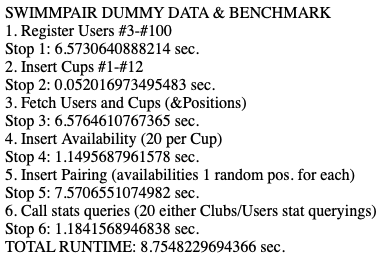
\includegraphics[scale=0.707]{img/app-benchmarking.png}
\fi
\chapter{Deployment}
Development of our application was done locally - using \textbf{Docker compose} to glue up three components necessary to sufficiently run our system - PHP runtime for web application, MySQL Database and Adminer. We have to, however, run our application in Kubernetes Cluster. \textbf{Service} and \textbf{Deployment} have to be written, Service for purposes of routing and taking care of container spawn addresses and Deployment to describe container replicas and approproate images. \textbf{Database} is run as separate entity within the Cluster.
\newline
\textbf{Running SwimmPair in Kubernetes Cluster:}
\par
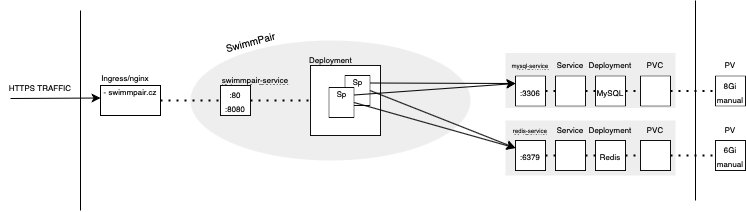
\includegraphics[scale=0.275]{img/swimmpair_deployment_k8s.png}
\section*{Dockerization of SwimmPair}
File called \textbf{Dockerfile} has to be created in the project folder.
\begin{lstlisting}
FROM thecodingmachine/php:7.4-v4-apache
COPY --chown=docker . /var/www/html
\end{lstlisting}
This image of Apache/PHP\footnote{thecodingmachine link} was chosen because it correctly dockerizes part of so-called LAMP stack. In order to build this image and push it into Dockerhub.com we run these commands:
\begin{lstlisting}
docker build -t stepanklos/swimmpair .
docker push stepanklos/swimmpair
\end{lstlisting}
This image is then pullable as stepanklos/swimmpair from Deployment.
\section*{Kubernetes}
We run X replicas on X Nodes in order to ensure reliability and uptime. 
\section*{Database and Redis}
As mentioned before, our application doesn't come with Database and Adminer, which have to be set up separately using persistent storage PV on which we write PVC and reference from deployment. 

%\chapter{User Manual}
\section{Public part}
Navigate the cups, users and statistics as a user interested in public information.
\subsection*{Application overview}
text about what is where
\subsection*{Cups printouts}
example screen
\subsection*{Public statistics}
example screen

\section{Administration}
SwimmPair administration after login has many options.
\newline
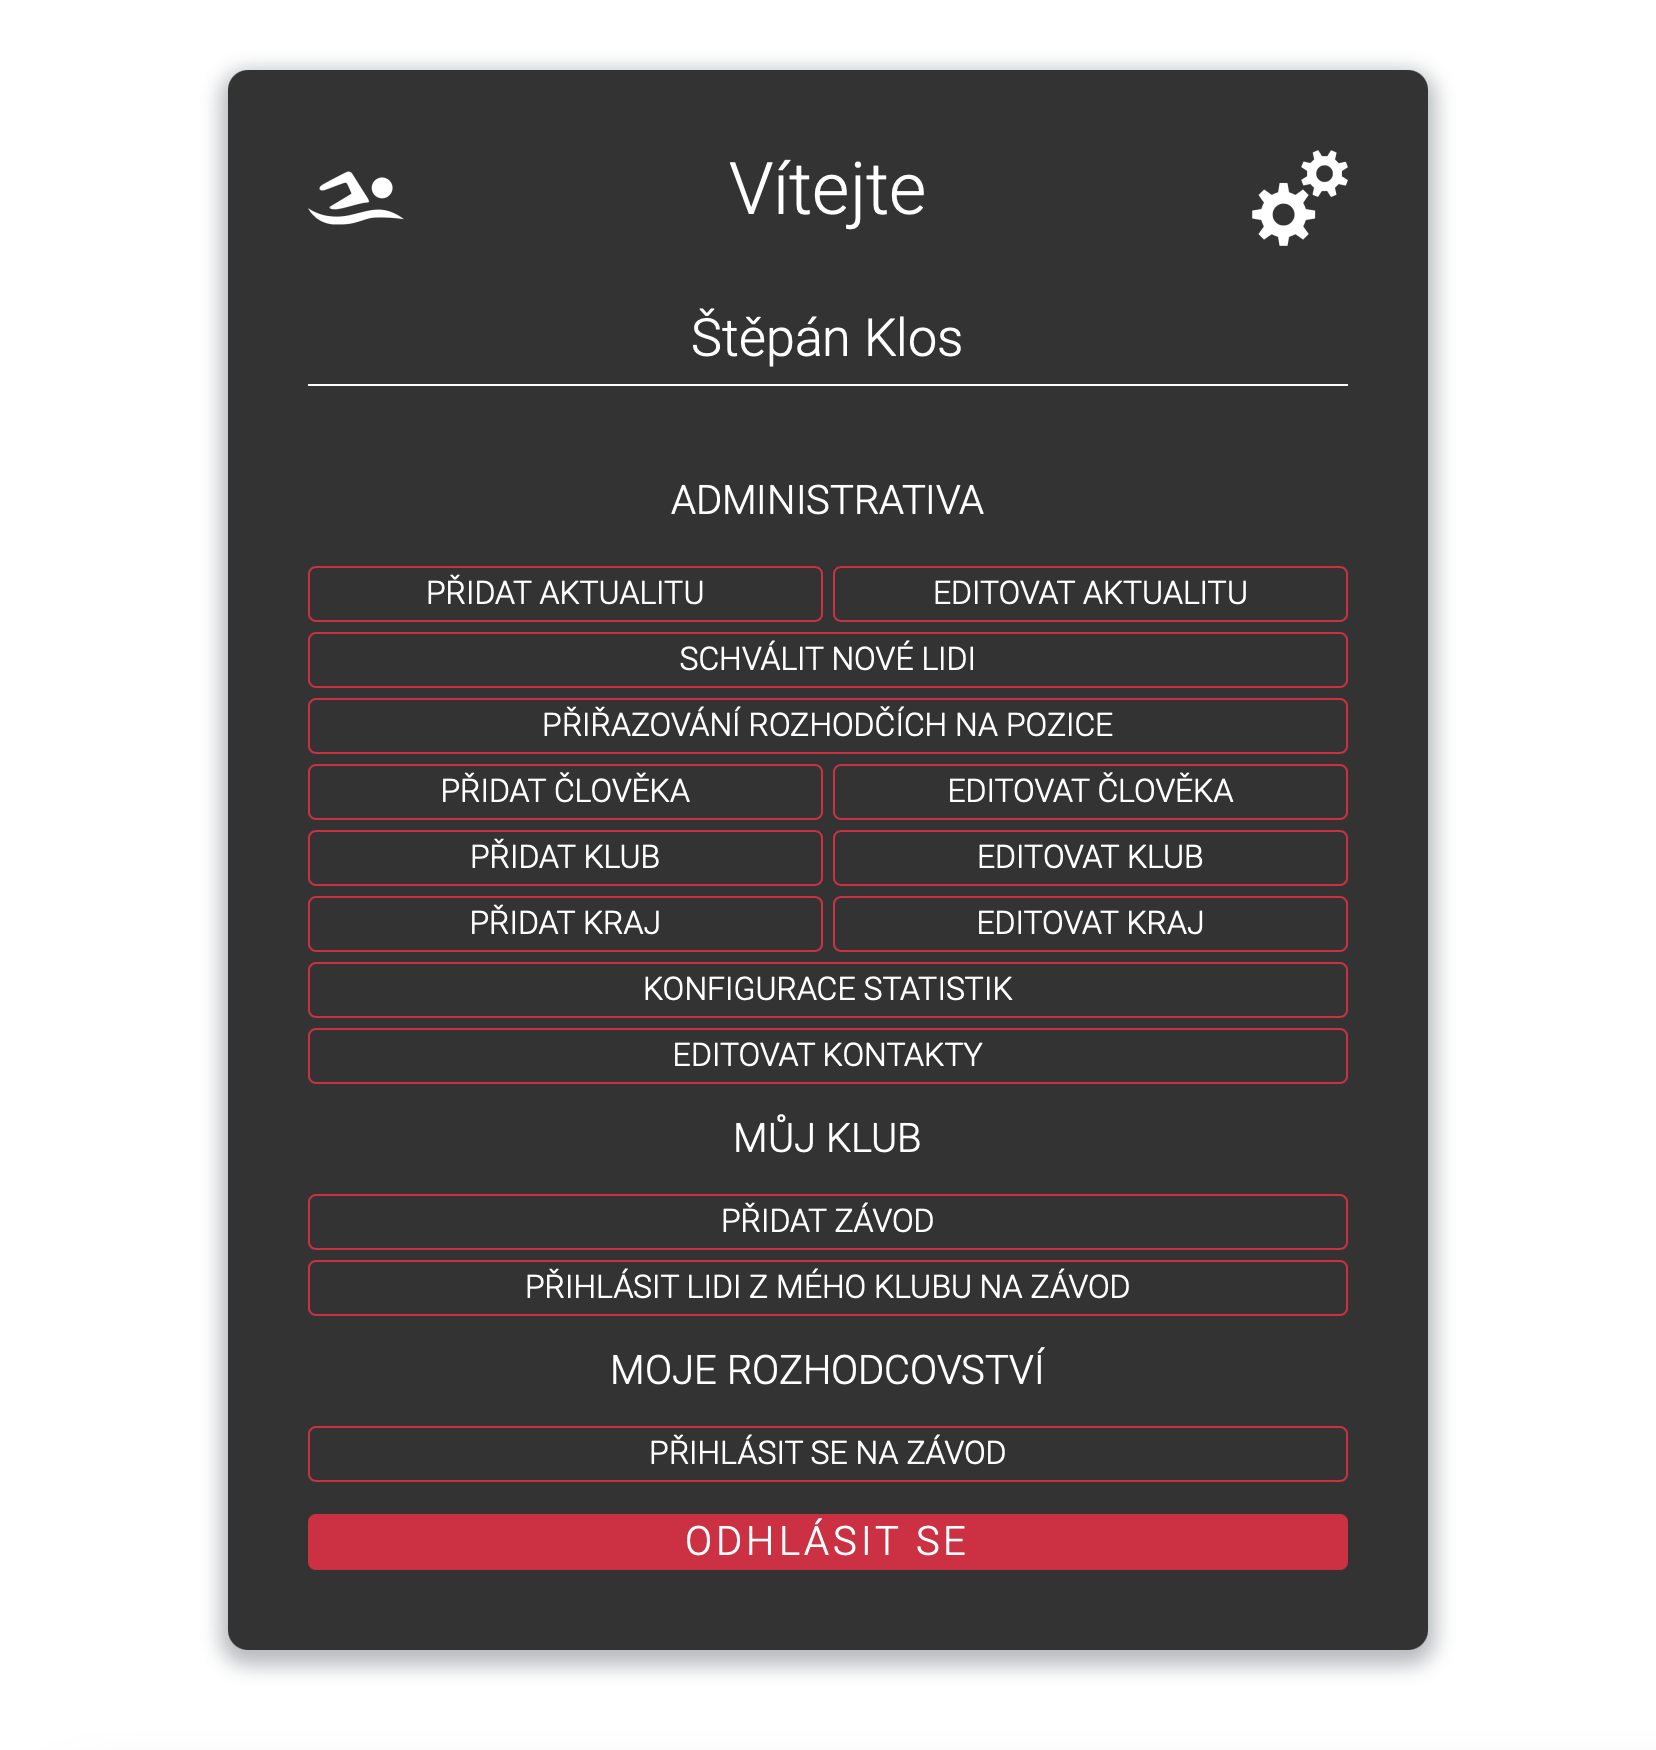
\includegraphics[scale=0.430]{img/admin_menu.png}
\subsection*{New Cup}
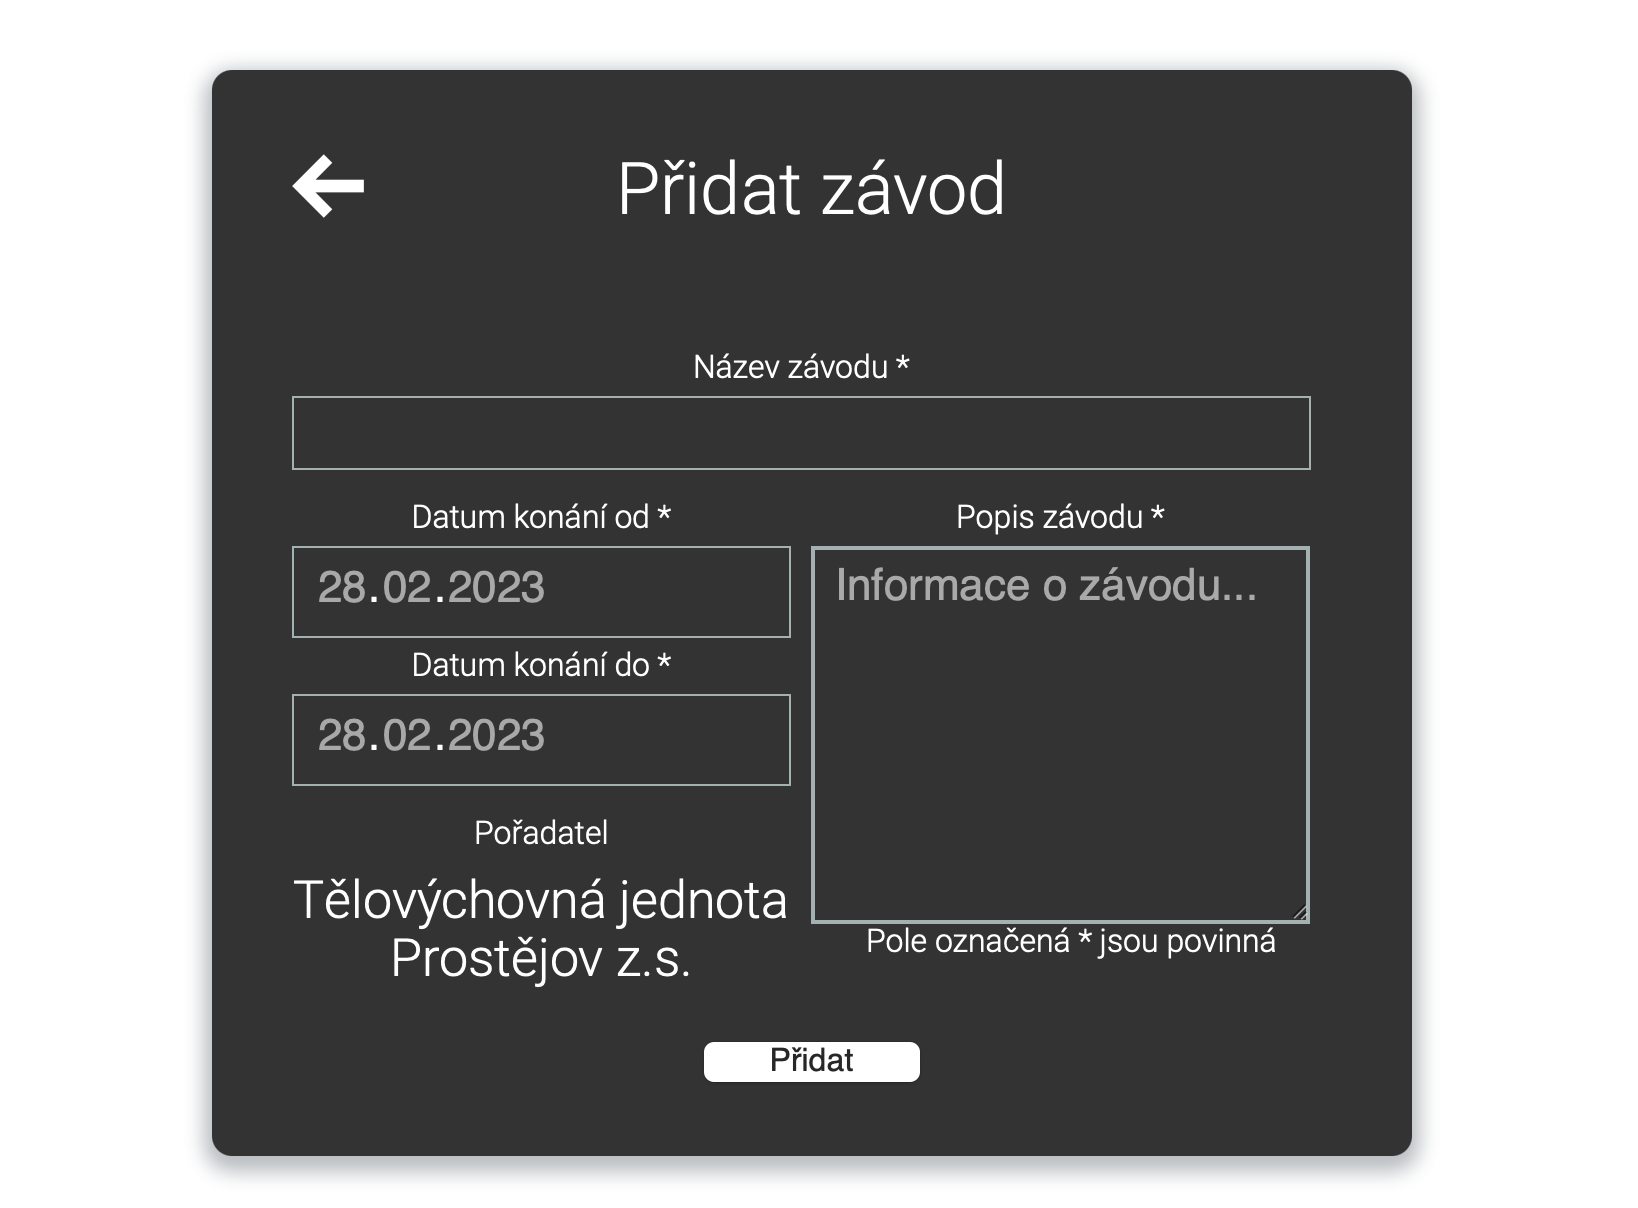
\includegraphics[scale=0.430]{img/admin_new_cup.png}
\subsection*{Participation availability}
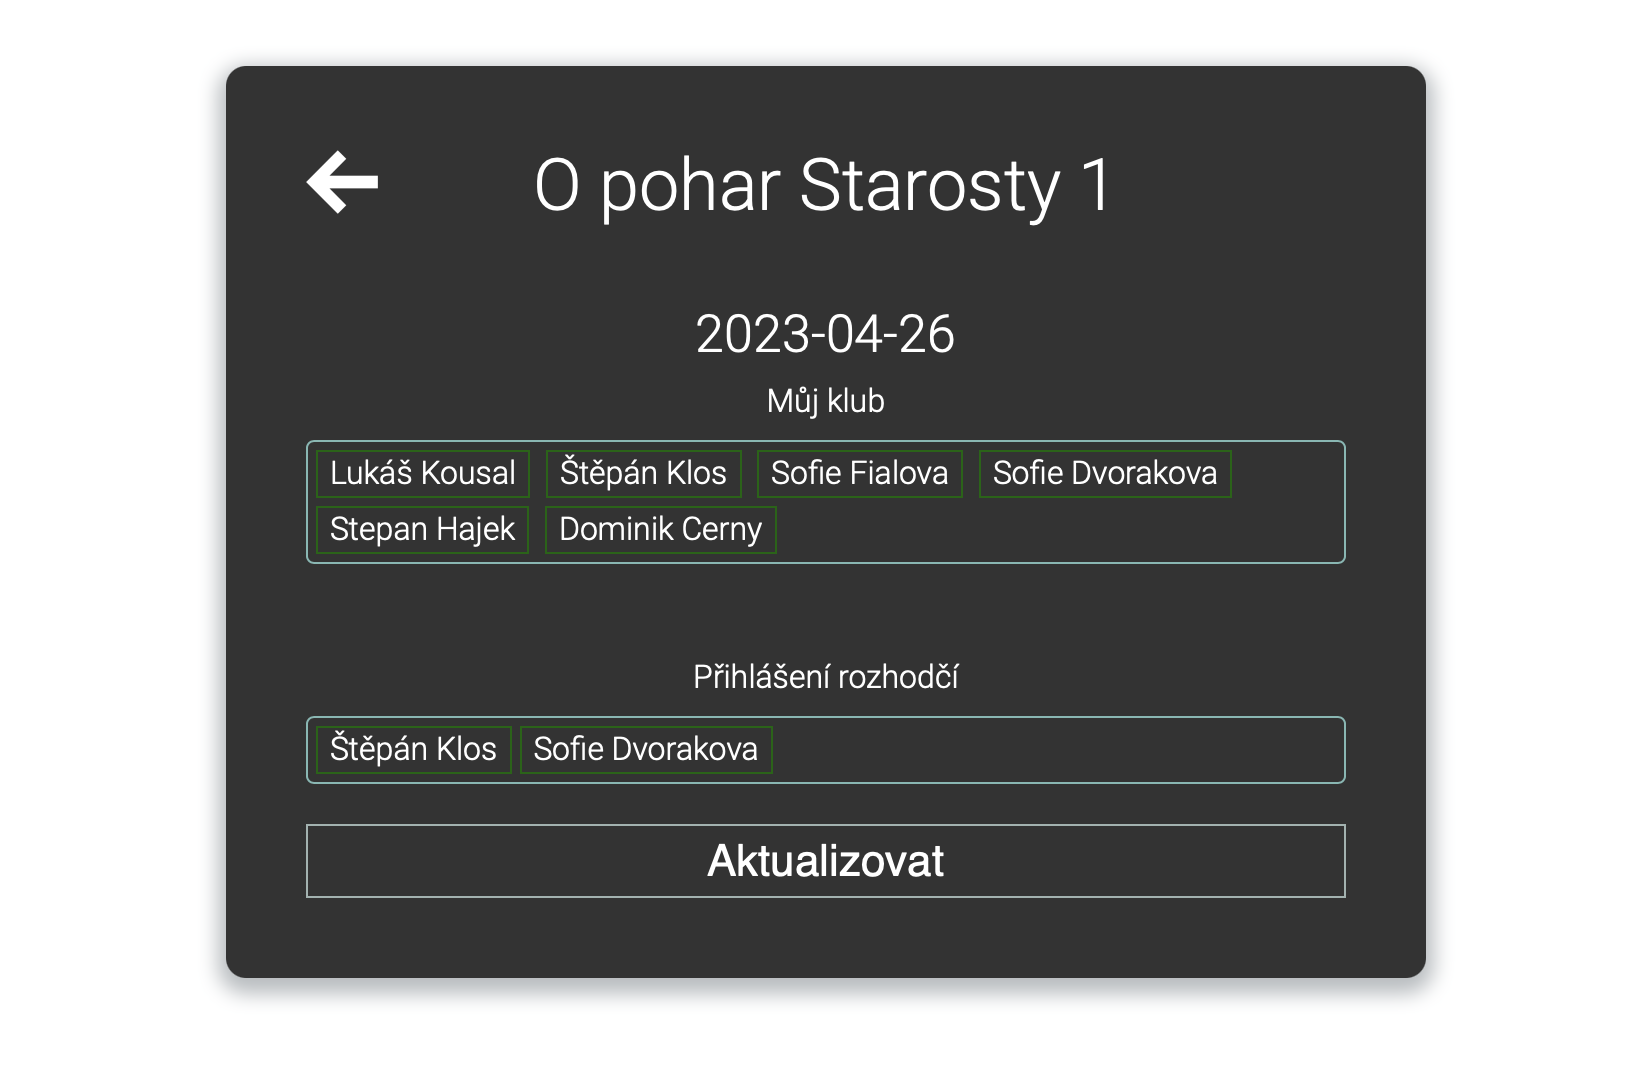
\includegraphics[scale=0.430]{img/admin_avail.png}
\subsection*{Pairing}
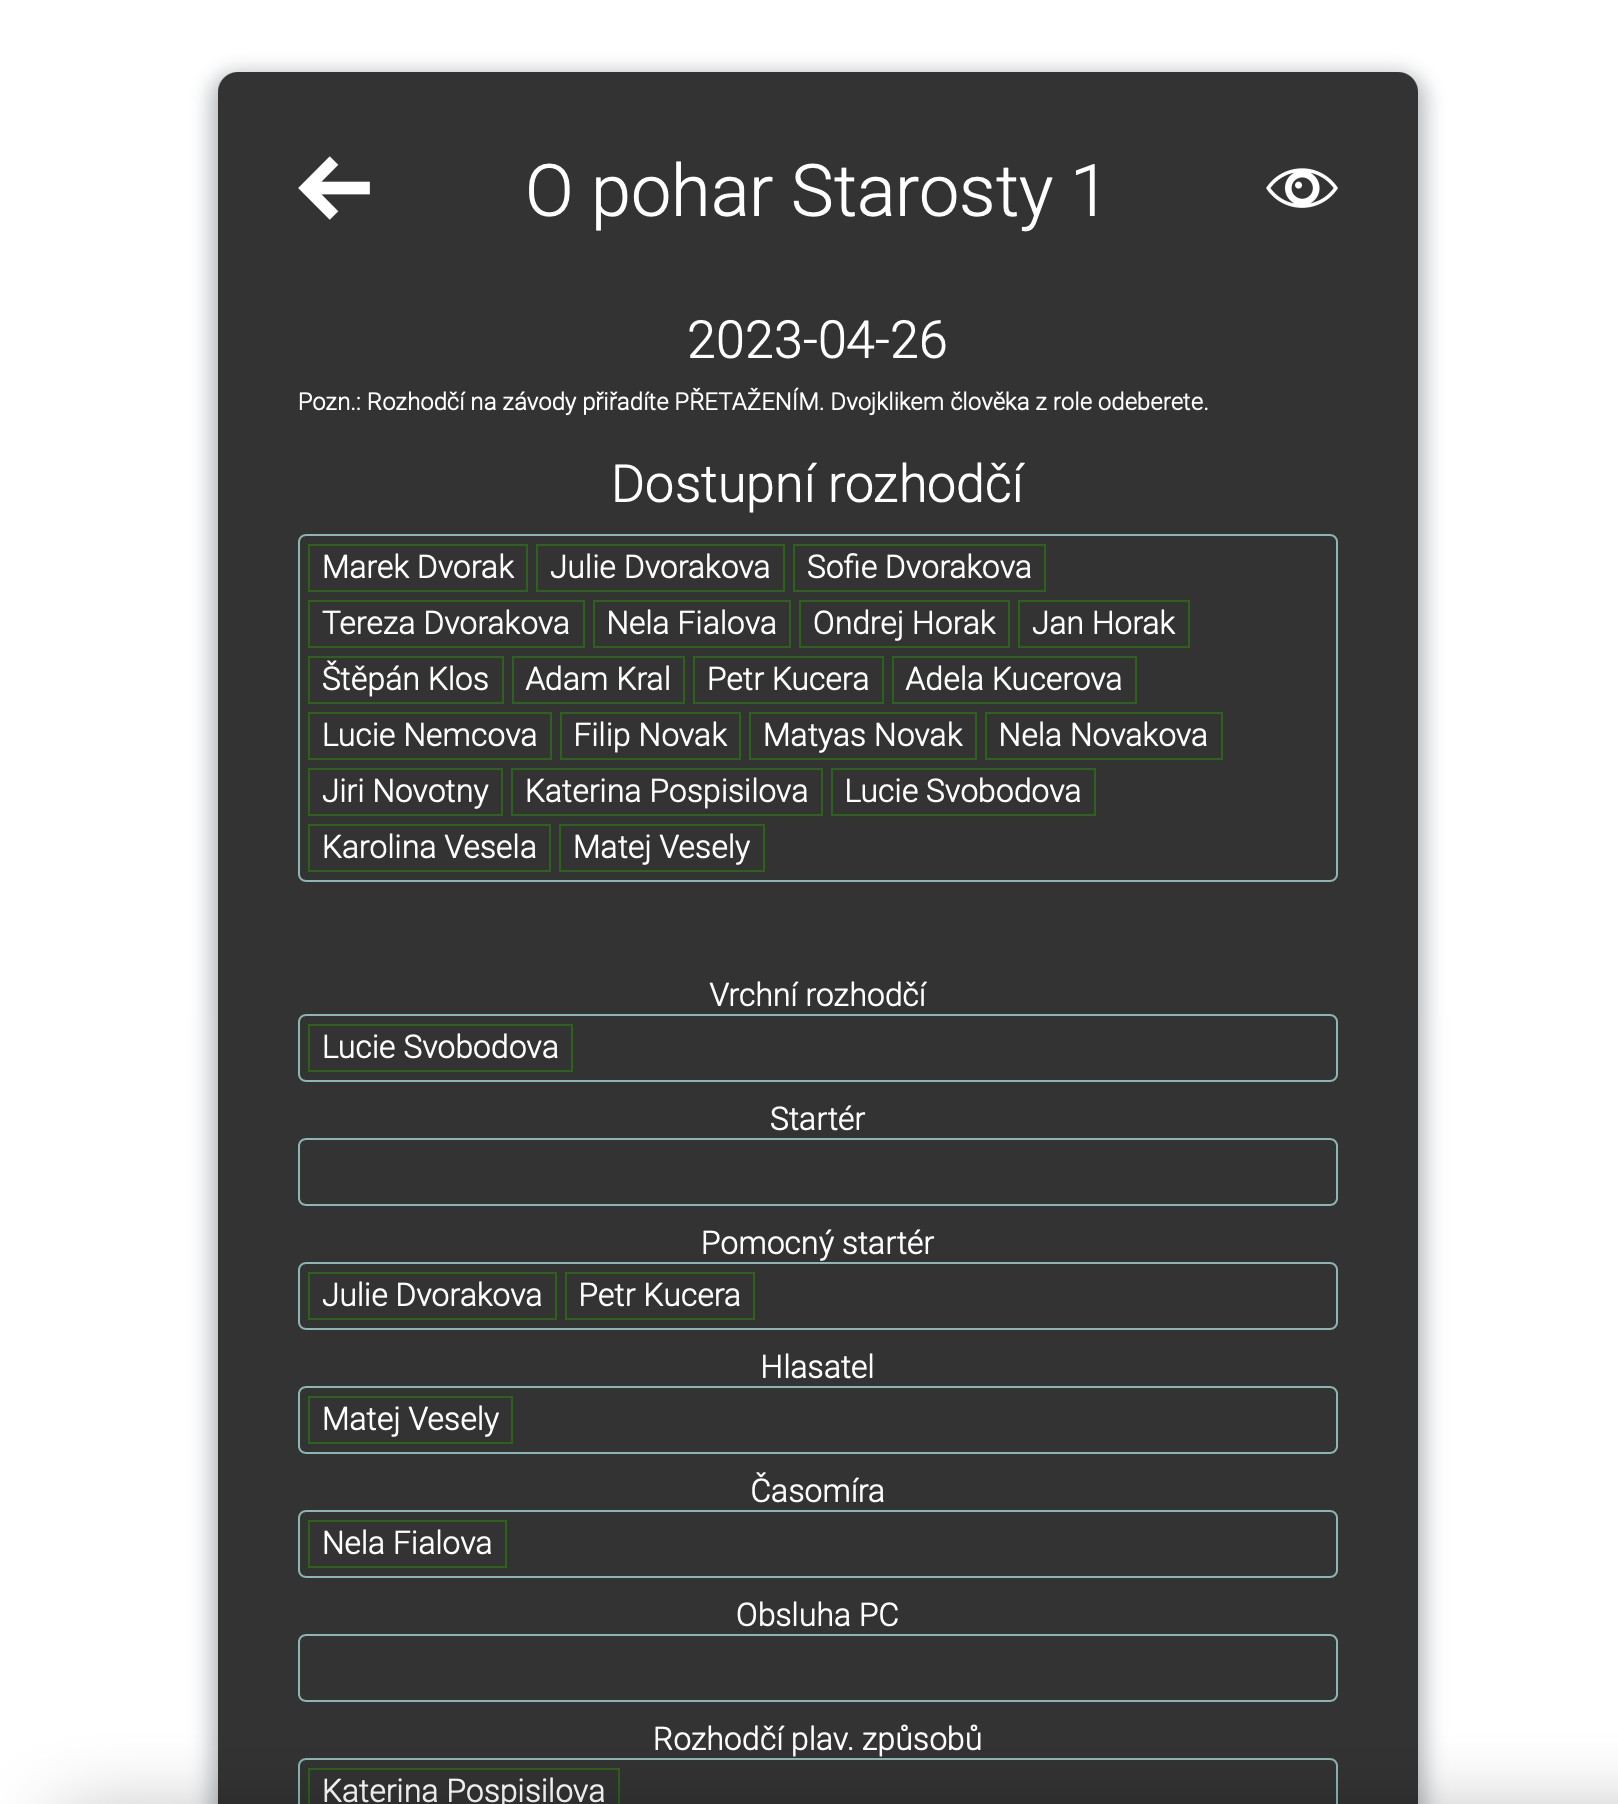
\includegraphics[scale=0.430]{img/admin_pairing.png}

\subsection*{Administrate SwimmPair as whole}

\chapter*{Conclusion}
The process of designing, developing, and shipping this web application was overall successful, although there are still some parts that could be improved or extended in the future. However, our system is ready for these changes and we have learned valuable lessons along the way.

In particular, the design and development process was not as straightforward as we had initially anticipated. Instead, it was an iterative process that required close collaboration with the system requester. The stages of iteration were roughly as follows.

\begin{enumerate}
\item Problem description and basic page layout programming (homepage, cup, user, club).
\item Formalization of the model and proper division of code into system objects and task functions.
\item Analysis of user and club data, additional pages for categorization purposes.
\item Addition of regions for further extensible hierarchization.
\item Major final refactoring of the database, backend, and testing with dummy data insertion and querying.
\item Cloud readiness, Docker image of the web application, and Kubernetes deployment.
\end{enumerate}

In the future, the system can be extended by adding new public pages, statistical queries, and administrative tasks. These modifications might involve adding new pages, adjusting the model, or making minor design changes. Thanks to the divided code, these changes can be easily accommodated and will reside in the project GitHub repository \footnote{\url{https://github.com/KlosStepan/SwimmPair-Www}}.

Overall, we are pleased with the outcome of this project and look forward to seeing it evolve further in the future.
\addcontentsline{toc}{chapter}{Conclusion}



%%% Bibliography
%%% Bibliography (literature used as a source)
%%%
%%% We employ bibTeX to construct the bibliography. It processes
%%% citations in the text (e.g., the \cite{...} macro) and looks up
%%% relevant entries in the bibliography.bib file.
%%%
%%% The \bibliographystyle command selects, which style will be used
%%% for references from the text. The argument in curly brackets is
%%% the name of the corresponding style file (*.bst). Both styles
%%% mentioned in this template are included in LaTeX distributions.

\bibliographystyle{plainnat}    %% Author (year)
% \bibliographystyle{unsrt}     %% [number]

\renewcommand{\bibname}{Bibliography}

%%% Generate the bibliography. Beware that if you cited no works,
%%% the empty list will be omitted completely.

\bibliography{bibliography}

%%% If case you prefer to write the bibliography manually (without bibTeX),
%%% you can use the following. Please follow the ISO 690 standard and
%%% citation conventions of your field of research.

 %\begin{thebibliography}{9}
%
% \bibitem{lamport94}
%   {\sc Lamport,} Leslie.
%   \emph{\LaTeX: A Document Preparation System}.
%   2nd edition.
%   Massachusetts: Addison Wesley, 1994.
%   ISBN 0-201-52983-1.
%
% \bibitem{einstein} 
%   Albert Einstein. 
%   \textit{Zur Elektrodynamik bewegter K{\"o}rper}. (German) 
%   [\textit{On the electrodynamics of moving bodies}]. 
%   Annalen der Physik, 322(10):891–921, 1905.
%
% \end{thebibliography}


%%% Figures used in the thesis (consider if this is needed)
\listoffigures

%%% Tables used in the thesis (consider if this is needed)
%%% In mathematical theses, it could be better to move the list of tables to the beginning of the thesis.
%\listoftables

%%% Abbreviations used in the thesis, if any, including their explanation
%%% In mathematical theses, it could be better to move the list of abbreviations to the beginning of the thesis.
\chapwithtoc{List of Abbreviations}

\begin{description}
  
  \item[CSPS] Cesky Svaz Plaveckych Sportu, \textit{Czech Swimming Federation} unites swimming clubs in the Czech Republic and provides competitions infrastructure and operations.
  
	\item[LAMP] Linux Apache MySQL PHP, standard stack for running applications.
	
	\item[SUS] System Usability Scale, is a standardized questionnaire consisting of 10 questions, which assesses the usability of a web application on a scale of 0-100. It provides a measure of how easy the application is to use, helping to identify areas for improvement.
	
  \item[DOKS] DigitalOcean Kubernetes, managed Kubernetes service by \url{https://www.digitalocean.com} with various products, scaling and functional options.
  
  \item[SwimmPair] Swimming Pairing, application that we developed and abbreviated and branded it like \textit{SwimmPair}.
  
  \item[UML] Unified Modeling Language, style of represent class relations between modelled objects in a functional design. 
  
  \item[CRUD] Create Read Update Delete, set of basic functions for performing I/O on dataset via Managers in our web application.
  
  \item[CI] Continuous Integration, is a software development practice that involves frequently integrating code changes from multiple developers into a shared repository. It aims to detect and resolve integration issues early by automatically building, testing, and validating code changes. This helps to ensure that the software is always in a working state and ready for deployment.  
  
  \item[K8s] is a shorthand way of writing "Kubernetes". The "8" in "K8s" represents the eight letters between the "K" and the "s" in "Kubernetes".
  
  \item[QA] auality assurance, refers to the process of ensuring that a product or service meets a certain level of quality and reliability.
	%\item[CIL] Common intermediate language, object oriented assembler defined by \emph{CLI} (also known as \emph{MSIL} or \emph{IL}).
	
	%\item[CLR] Common language runtime, virtual machine implementing the execution engine specified by \emph{CLI}.
	
	%\item[DLR] Dynamic language runtime, set of libraries providing compiler and runtime services for dynamic languages build on top of \emph{CLR}.
	
	%\item[AST] Abstract syntax tree, structured representation of the source code.
	
	%\item[CFG] Control flow graph, a semantic graph representing a method.
	
\end{description}
%%% Attachments to the bachelor thesis, if any. Each attachment must be
%%% referred to at least once from the text of the thesis. Attachments
%%% are numbered.
%%%
%%% The printed version should preferably contain attachments, which can be
%%% read (additional tables and charts, supplementary text, examples of
%%% program output, etc.). The electronic version is more suited for attachments
%%% which will likely be used in an electronic form rather than read (program
%%% source code, data files, interactive charts, etc.). Electronic attachments
%%% should be uploaded to SIS and optionally also included in the thesis on a~CD/DVD.
%%% Allowed file formats are specified in provision of the rector no. 72/2017.
%\appendix
%\chapter{Attachments}

%\section{First Attachment}

\openright
\end{document}
